\documentclass{article}


\usepackage[margin=1.2in]{geometry}
\usepackage{parskip}

% \relax % Controls
    \newif\ifmarginprooflinks
    	\marginprooflinkstrue
    	% \marginprooflinksfalse

\relax % Bibliography, etc
	\usepackage[american]{babel}
	\usepackage{csquotes}
	\usepackage[backend=biber, style=authoryear]{biblatex}
	\DeclareLanguageMapping{american}{american-apa}
	% \usepackage[backend=biber,style=authoryear,hyperref=true]{biblatex}
	% \addbibresource{refs.bib}
	% \addbibresource{conf.bib}

	\DeclareFieldFormat{citehyperref}{%
	  \DeclareFieldAlias{bibhyperref}{noformat}% Avoid nested links
	  \bibhyperref{#1}}

	\DeclareFieldFormat{textcitehyperref}{%
	  \DeclareFieldAlias{bibhyperref}{noformat}% Avoid nested links
	  \bibhyperref{%
	    #1%
	    \ifbool{cbx:parens}
	      {\bibcloseparen\global\boolfalse{cbx:parens}}
	      {}}}

	\savebibmacro{cite}
	\savebibmacro{textcite}

	\renewbibmacro*{cite}{%
	  \printtext[citehyperref]{%
	    \restorebibmacro{cite}%
	    \usebibmacro{cite}}}

	\renewbibmacro*{textcite}{%
	  \ifboolexpr{
	    ( not test {\iffieldundef{prenote}} and
	      test {\ifnumequal{\value{citecount}}{1}} )
	    or
	    ( not test {\iffieldundef{postnote}} and
	      test {\ifnumequal{\value{citecount}}{\value{citetotal}}} )
	  }
	    {\DeclareFieldAlias{textcitehyperref}{noformat}}
	    {}%
	  \printtext[textcitehyperref]{%
	    \restorebibmacro{textcite}%
	    \usebibmacro{textcite}}}

	\DeclareCiteCommand{\brakcite}
	  {\usebibmacro{prenote}}
	  {\usebibmacro{citeindex}%
	   \printtext[bibhyperref]{[\usebibmacro{cite}]}}
	  {\multicitedelim}
	  {\usebibmacro{postnote}}

\relax % Standard Packages
    \usepackage[dvipsnames]{xcolor}
    % \usepackage[utf8]{inputenc}
    \usepackage{mathtools}
    \usepackage{amssymb}
		\DeclareMathSymbol{\shortminus}{\mathbin}{AMSa}{"39}
    % \usepackage{parskip}
    % \usepackage{algorithm}
    \usepackage{bbm}
	\usepackage{lmodern}
	% \usepackage{times}
    \usepackage{faktor}
    % \usepackage{booktabs}
	% \usepackage[margin=1in]{geometry}
    \usepackage{graphicx}
    \usepackage{scalerel}
    \usepackage{enumitem}
    \usepackage{nicefrac}\let\nf\nicefrac

    % \usepackage{color}
    %\usepackage{stmaryrd}
    \usepackage{hyperref} % Load before theorems...
        \hypersetup{colorlinks=true, linkcolor=blue!75!black, urlcolor=magenta, citecolor=green!50!black}

\usepackage{tikz}
	\usetikzlibrary{positioning,fit,calc, decorations, arrows, shapes, shapes.geometric}
	\usetikzlibrary{cd}

	%%%%%%%%%%%%
	\tikzset{AmpRep/.style={ampersand replacement=\&}}
	\tikzset{center base/.style={baseline={([yshift=-.8ex]current bounding box.center)}}}
	\tikzset{paperfig/.style={center base,scale=0.9, every node/.style={transform shape}}}

	% Node Stylings
	\tikzset{dpadded/.style={rounded corners=2, inner sep=0.7em, draw, outer sep=0.3em, fill={black!50}, fill opacity=0.08, text opacity=1}}
	\tikzset{dpad0/.style={outer sep=0.05em, inner sep=0.3em, draw=gray!75, rounded corners=4, fill=black!08, fill opacity=1, align=center}}
	\tikzset{dpadinline/.style={outer sep=0.05em, inner sep=2.5pt, rounded corners=2.5pt, draw=gray!75, fill=black!08, fill opacity=1, align=center, font=\small}}

 	\tikzset{dpad/.style args={#1}{every matrix/.append style={nodes={dpadded, #1}}}}
	\tikzset{light pad/.style={outer sep=0.2em, inner sep=0.5em, draw=gray!50}}

	\tikzset{arr/.style={draw, ->, thick, shorten <=3pt, shorten >=3pt}}
	\tikzset{arr0/.style={draw, ->, thick, shorten <=0pt, shorten >=0pt}}
	\tikzset{arr1/.style={draw, ->, thick, shorten <=1pt, shorten >=1pt}}
	\tikzset{arr2/.style={draw, ->, thick, shorten <=2pt, shorten >=2pt}}

	\newcommand\cmergearr[5][]{
		\draw[arr, #1, -] (#2) -- (#5) -- (#3);
		\draw[arr, #1, shorten <=0] (#5) -- (#4);
		}
	\newcommand\mergearr[4][]{
		\coordinate (center-#2#3#4) at (barycentric cs:#2=1,#3=1,#4=1.2);
		\cmergearr[#1]{#2}{#3}{#4}{center-#2#3#4}
		}
	\newcommand\cunmergearr[5][]{
		\draw[arr, #1, -, shorten >=0] (#2) -- (#5);
		\draw[arr, #1, shorten <=0] (#5) -- (#3);
		\draw[arr, #1, shorten <=0] (#5) -- (#4);
		}
	\newcommand\unmergearr[4][]{
		\coordinate (center-#2#3#4) at (barycentric cs:#2=1.2,#3=1,#4=1);
		\cunmergearr[#1]{#2}{#3}{#4}{center-#2#3#4}
		}

\usepackage{amsthm,thmtools} % Theorem Macros
	\usepackage[noabbrev,nameinlink,capitalize]{cleveref}
    \theoremstyle{plain}
    \newtheorem{theorem}{Theorem}
	\newtheorem{coro}{Corollary}[theorem]
    \newtheorem{prop}[theorem]{Proposition}
    \newtheorem{conj}[theorem]{Conjecture}
    \newtheorem{claim}{Claim}
    \newtheorem{remark}{Remark}
    \newtheorem{lemma}[theorem]{Lemma}
    \theoremstyle{definition}
    % \newtheorem{defn}{Definition}
    % \declaretheorem[name=Definition]{defn}
    \declaretheorem[name=Definition, qed=$\square$]{defn}
    \declaretheorem[name=Example, qed=$\triangle$]{example}

	\crefname{defn}{Definition}{Definitions}
	\crefname{prop}{Proposition}{Propositions}
    \crefname{issue}{Issue}{Issues}

\relax %%%%%%%%% GENERAL MACROS %%%%%%%%
    \let\Horig\H
	\let\H\relax
	\DeclareMathOperator{\H}{\mathrm{H}} % Entropy
	\DeclareMathOperator{\I}{\mathrm{I}} % Information
	\DeclareMathOperator*{\Ex}{\mathbb{E}} % Expectation
	\DeclareMathOperator*{\EX}{\scalebox{1.5}{$\mathbb{E}$}}

    \newcommand{\mat}[1]{\mathbf{#1}}
    \DeclarePairedDelimiterX{\infdivx}[2]{(}{)}{%
		#1\;\delimsize\|\;#2%
	}
	\newcommand{\thickD}{I\mkern-8muD}
	\newcommand{\kldiv}{\thickD\infdivx}
	\newcommand{\tto}{\rightarrow\mathrel{\mspace{-15mu}}\rightarrow}

	\newcommand{\datadist}[1]{\Pr\nolimits_{#1}}
	% \newcommand{\datadist}[1]{p_\text{data}}

	\makeatletter
	\newcommand{\subalign}[1]{%
	  \vcenter{%
	    \Let@ \restore@math@cr \default@tag
	    \baselineskip\fontdimen10 \scriptfont\tw@
	    \advance\baselineskip\fontdimen12 \scriptfont\tw@
	    \lineskip\thr@@\fontdimen8 \scriptfont\thr@@
	    \lineskiplimit\lineskip
	    \ialign{\hfil$\m@th\scriptstyle##$&$\m@th\scriptstyle{}##$\hfil\crcr
	      #1\crcr
	    }%
	  }%
	}
	\makeatother
	\newcommand\numberthis{\addtocounter{equation}{1}\tag{\theequation}}

\relax %%%%%%%%%   PDG  MACROS   %%%%%%%%
	\newcommand{\ssub}[1]{_{\!_{#1}\!}}
	% \newcommand{\bp}[1][L]{\mat{p}_{\!_{#1}\!}}
	% \newcommand{\bP}[1][L]{\mat{P}_{\!_{#1}\!}}
	\newcommand{\bp}[1][L]{\mat{p}\ssub{#1}}
	\newcommand{\bP}[1][L]{\mat{P}\ssub{#1}}
	\newcommand{\V}{\mathcal V}
	\newcommand{\N}{\mathcal N}
	\newcommand{\Ed}{\mathcal E}

    \newcommand{\balpha}{\boldsymbol\alpha}
    \newcommand{\bbeta}{\boldsymbol\beta}

	\DeclareMathAlphabet{\mathdcal}{U}{dutchcal}{m}{n}
	\DeclareMathAlphabet{\mathbdcal}{U}{dutchcal}{b}{n}
	\newcommand{\dg}[1]{\mathbdcal{#1}}
	\newcommand{\PDGof}[1]{{\dg M}_{#1}}
	\newcommand{\UPDGof}[1]{{\dg N}_{#1}}
	\newcommand\VFE{\mathit{V\mkern-4mu F\mkern-4.5mu E}}

	\newcommand\Inc{\mathit{Inc}}
	\newcommand{\IDef}[1]{\mathit{IDef}_{\!#1}}
	% \newcommand{\ed}[3]{%
	% 	\mathchoice%
	% 	{#2\overset{\smash{\mskip-5mu\raisebox{-3pt}{${#1}$}}}{\xrightarrow{\hphantom{\scriptstyle {#1}}}} #3} %display style
	% 	{#2\overset{\smash{\mskip-5mu\raisebox{-3pt}{$\scriptstyle {#1}$}}}{\xrightarrow{\hphantom{\scriptstyle {#1}}}} #3}% text style
	% 	{#2\overset{\smash{\mskip-5mu\raisebox{-3pt}{$\scriptscriptstyle {#1}$}}}{\xrightarrow{\hphantom{\scriptscriptstyle {#1}}}} #3} %script style
	% 	{#2\overset{\smash{\mskip-5mu\raisebox{-3pt}{$\scriptscriptstyle {#1}$}}}{\xrightarrow{\hphantom{\scriptscriptstyle {#1}}}} #3}} %scriptscriptstyle
	\newcommand{\ed}[3]{#2%
	  \overset{\smash{\mskip-5mu\raisebox{-1pt}{$\scriptscriptstyle
	        #1$}}}{\rightarrow} #3}

    \newcommand{\nhphantom}[2]{\sbox0{\kern-2%
		\nulldelimiterspace$\left.\delimsize#1\vphantom{#2}\right.$}\hspace{-.97\wd0}}
		% \nulldelimiterspace$\left.\delimsize#1%
		% \vrule depth\dp#2 height \ht#2 width0pt\right.$}\hspace{-.97\wd0}}
	\makeatletter
	\newsavebox{\abcmycontentbox}
	\newcommand\DeclareDoubleDelim[5]{
	    \DeclarePairedDelimiterXPP{#1}[1]%
			{% box must be saved in this pre code
				\sbox{\abcmycontentbox}{\ensuremath{##1}}%
			}{#2}{#5}{}%
		    %%% Correct spacing, but doesn't work with externalize.
			% {\nhphantom{#3}{##1}\hspace{1.2pt}\delimsize#3\mathopen{}##1\mathclose{}\delimsize#4\hspace{1.2pt}\nhphantom{#4}{##1}}
			%%% Fast, but wrong spacing.
			% {\nhphantom{#3}{~}\hspace{1.2pt}\delimsize#3\mathopen{}##1\mathclose{}\delimsize#4\hspace{1.2pt}\nhphantom{#4}{~}}
			%%% with savebox.
		    {%
				\nhphantom{#3}{\usebox\abcmycontentbox}%
				\hspace{1.2pt} \delimsize#3%
				\mathopen{}\usebox{\abcmycontentbox}\mathclose{}%
				\delimsize#4\hspace{1.2pt}%
				\nhphantom{#4}{\usebox\abcmycontentbox}%
			}%
	}
	\makeatother
	\DeclareDoubleDelim
		\SD\{\{\}\}
	\DeclareDoubleDelim
		\bbr[[]]
	% \DeclareDoubleDelim
	% 	\aar\langle\langle\rangle\rangle
	\makeatletter
	\newsavebox{\aar@content}
	\newcommand\aar{\@ifstar\aar@one@star\aar@plain}
	\newcommand\aar@one@star{\@ifstar\aar@resize{\aar@plain*}}
	\newcommand\aar@resize[1]{\sbox{\aar@content}{#1}\scaleleftright[3.8ex]
		{\Biggl\langle\!\!\!\!\Biggl\langle}{\usebox{\aar@content}}
		{\Biggr\rangle\!\!\!\!\Biggr\rangle}}
	\DeclareDoubleDelim
		\aar@plain\langle\langle\rangle\rangle
	\makeatother


	% \DeclarePairedDelimiterX{\aar}[1]{\langle}{\rangle}
	% 	{\nhphantom{\langle}{#1}\hspace{1.2pt}\delimsize\langle\mathopen{}#1\mathclose{}\delimsize\rangle\hspace{1.2pt}\nhphantom{\rangle}{#1}}

\relax %%%%% restatables and links
	% \usepackage{xstring} % for expandarg
	\usepackage{xpatch}
	\makeatletter
	\xpatchcmd{\thmt@restatable}% Edit \thmt@restatable
	   {\csname #2\@xa\endcsname\ifx\@nx#1\@nx\else[{#1}]\fi}% Replace this code
	   % {\ifthmt@thisistheone\csname #2\@xa\endcsname\typeout{oiii[#1;#2\@xa;#3;\csname thmt@stored@#3\endcsname]}\ifx\@nx#1\@nx\else[#1]\fi\else\csname #2\@xa\endcsname\fi}% with this code
	   {\ifthmt@thisistheone\csname #2\@xa\endcsname\ifx\@nx#1\@nx\else[{#1}]\fi
	   \else\fi}
	   {}{\typeout{FIRST PATCH TO THM RESTATE FAILED}} % execute on success/failure
	\xpatchcmd{\thmt@restatable}% A second edit to \thmt@restatable
	   {\csname end#2\endcsname}
	   {\ifthmt@thisistheone\csname end#2\endcsname\else\fi}
	   {}{\typeout{FAILED SECOND THMT RESTATE PATCH}}

	% \def\onlyaftercolon#1:#2{#2}
	\newcommand{\recall}[1]{\medskip\par\noindent{\bf \Cref{thmt@@#1}.} \begingroup\em \noindent
	   \expandafter\csname#1\endcsname* \endgroup\par\smallskip}

   	\setlength\marginparwidth{1.55cm}
	\newenvironment{linked}[3][]{%
		\def\linkedproof{#3}%
		\def\linkedtype{#2}%
		% \reversemarginpar
		% \marginpar{%
		% \vspace{1.1em}
		% % \hspace{2em}
		% 	% \raggedleft
		% 	\raggedright
		% 	\hyperref[proof:\linkedproof]{%
		% 	\color{blue!50!white}
		% 	\scaleleftright{$\Big[$}{\,{\small\raggedleft\tt\begin{tabular}{@{}c@{}} proof of \\\linkedtype~\ref*{\linkedtype:\linkedproof}\end{tabular}}\,}{$\Big]$}}
		% 	}%
        % \restatable[#1]{#2}{#2:#3}\label{#2:#3}%
		\ifmarginprooflinks
		\marginpar{%
			% \vspace{-3em}% %% for bottom
			\vspace{1.5em}
			\centering%
			\hyperref[proof:\linkedproof]{%
            % \hyperref[proof:#3]{
			\color{blue!30!white}%
			\scaleleftright{$\Big[$}{\,\mbox{\footnotesize\centering\tt\begin{tabular}{@{}c@{}}
				% proof of \\\,\linkedtype~\ref*{\linkedtype:\linkedproof}
				link to\\[-0.15em]
				proof
			\end{tabular}}\,}{$\Big]$}}~
			}%
		\fi
        \restatable[#1]{#2}{#2:#3}\label{#2:#3}%
        }%
		{\endrestatable%
		}
	\makeatother
		\newcounter{proofcntr}
		\newenvironment{lproof}{\begin{proof}\refstepcounter{proofcntr}}{\end{proof}}

		\usepackage{cancel}
		\newcommand{\Cancel}[2][black]{{\color{#1}\cancel{\color{black}#2}}}

		\usepackage{tcolorbox}
		\tcbuselibrary{most}
		\tcolorboxenvironment{lproof}{
			% fonttitle=\bfseries,
			% top=0.5em,
			enhanced,
			parbox=false,
			boxrule=0pt,
			frame hidden,
			borderline west={4pt}{0pt}{blue!20!black!40!white},
			% coltext={blue!20!black!60!white},
			colback={blue!20!black!05!white},
			sharp corners,
			breakable,
			% bottomsep at break=4cm,
			% enlarge bottom at break by=-4cm,
			% topsep at break=3cm,
			% enlarge top at break by=-3cm
		}
		% \usepackage[framemethod=TikZ]{mdframed}
		% \surroundwithmdframed[ % lproof
		% 	   topline=false,
		% 	   linewidth=3pt,
		% 	   linecolor=gray!20!white,
		% 	   rightline=false,
		% 	   bottomline=false,
		% 	   leftmargin=0pt,
		% 	   % innerleftmargin=5pt,
		% 	   skipabove=\medskipamount,
		% 	   skipbelow=\medskipamount
		% 	]{lproof}
	%oli16: The extra space was because there was extra space in the paragraph, not
	%because this length was too big. By breaking arrays, everything will be better.
	\newcommand{\begthm}[3][]{\begin{#2}[{name=#1},restate=#3,label=#3]}

\relax %TODOs and footnotes
    \newcommand{\TODO}[1][INCOMPLETE]{{\centering\Large\color{red}$\langle$~\texttt{#1}~$\rangle$\par}}
    \newcommand{\dfootnote}[1]{%
        \let\oldthefootnote=\thefootnote%
        % \addtocounter{footnote}{-1}%
		\setcounter{footnote}{999}
        \renewcommand{\thefootnote}{\textdagger}%
        \footnote{#1}%
        \let\thefootnote=\oldthefootnote%
    }
	\newcommand{\dfootnotemark}{
		\footnotemark[999]
	}


% \usepackage[framemethod=TikZ]{mdframed}
% \colorlet{color1}{Emerald}
% \colorlet{color3}{color1>wheel,2,3}
% \colorlet{pinkish}{color3!25!magenta}
\definecolor{brownish}{rgb}{0.5, 0.2, 0.1}
% \newmdenv[roundcorner=5pt, 
%     backgroundcolor=brownish!20!white,
%     % frametitle={$\langle$under construction$\rangle$},
%     frametitle={$\langle$incomplete or buggy$\rangle$},
%     frametitlerule=false,
%     innertopmargin=3pt, frametitlebelowskip=1ex, frametitleaboveskip=1ex,
%     frametitlebackgroundcolor=brownish!40!white,
%     skipabove=1em,skipbelow=1em,
%     frametitlefont={\scshape},leftmargin=-10pt, rightmargin=-10pt]
% 		{wip}
\newtcolorbox{wip}{%
    colback=brownish!20!white,%
    % frametitle={$\langle$under construction$\rangle$},
    title={$\langle$incomplete or buggy$\rangle$},%
    enhanced jigsaw,
    breakable,
    % frametitlerule=false,
    % innertopmargin=3pt, frametitlebelowskip=1ex, frametitleaboveskip=1ex,
    colframe=brownish!40!white,%
    % skipabove=1em,skipbelow=1em,
    % frametitlefont={\scshape},leftmargin=-10pt, rightmargin=-10pt
}
        
% \tcolorboxenvironment{example}{
\newtcolorbox[use counter=example]{examplex}{
        fonttitle=\bfseries,
        % empty,
        enhanced jigsaw,
        title={Example \thetcbcounter.},
        before=\par\medskip\noindent,
        % top=0.5em,
        % enhanced,
        parbox=false,
        % boxrule=0pt,
        % frame hidden,
        % borderline west={4pt}{0pt}{green!20!black!40!white},
        % coltext={blue!20!black!60!white},
        % colback={blue!20!black!05!white},
        colback=white,
        sharp corners,
        breakable,
        % bottomsep at break=4cm,
        % enlarge bottom at break by=-4cm,
        % topsep at break=3cm,
        % enlarge top at break by=-3cm
    }

\input{confidence-preamble}

\addbibresource{conf.bib}

% \newcommand{\ext}[1]{\mathcal M#1} %measures over phi
% \newcommand{\ext}[1]{\mathbb R^{#1}_{\mathrm{fin}}} % finite measures over phi
\newcommand{\ext}[1]{\overline #1} %  measures over phi
\newcommand{\Unif}{\mathrm{Unif}}

\DeclareMathOperator{\supp}{\mathrm{Supp}}


\begin{document}

\begin{center}
    \Large\scshape
    % Confidence: How to think of partial updates
    % Confidence, the
    Updating with Variable Confidence
    % Partial Updates
    % (Belief Opacity?)
\end{center}
\bigskip

\tableofcontents

% You have confidence in a piece of information.
% The word ``confidence'' is sometimes used to stand in for a piece of information.
% While high confidence in an event is much like high probability in the event, low confidence in the event and low probability are entriely different.

\section{Introduction}

Properties of Confidence
\begin{enumerate}[nosep]
    \item Updating with zero confidence leaves belief state unchanged.
    \item Updating with infinite confidence causes you to (permanently) gain a certainty.
    \item
\end{enumerate}


\section{The Opacity Analogy}

% \begin{minipage}{0.48\linewidth}

    So far as a computer display is concerned, what ultimately matters are pixel colors.
    And yet, in the standard representation of a color color, only three of the four bytes actually encodes color information; the last one describes opacity---in some sense, a \emph{confidence} in the color.
    % Far from an oversight, this enables the possibility of suggest a color with less than complete confidence is incredibly useful.
    % The result is an ability to suggest a color with less than complete confidence.
    This enables a great deal in graphics: intricate digital art, via semantically meaningful layers,
        visual effects such as fire and fog that do not need to be modeled jointly with their surroundings.
    % This is not an oversight; working with translucency can be incredibly valuable.
     % porgrams enables .%
        % \footnote{just as higher-level programming languages enable programmers to build larger projects by giving larger-scale structure}



% \end{minipage}
% \hfill
% \begin{minipage}{0.48\linewidth}
    So far as statistical models are concerned, what ultimately matters are probabilities of events.
    But that doesn't appear to

\section{Update Rules: Changes in Confidence}
\def\X{\mathcal X}

% We now describe our formal approach, in which
% We now proceed with the formal details.

% maybe??
% Let $\Phi$ be the set of statements about $X$ --- that is, the things one can have confidnce in.
Consider a space $\Theta$
of possible belief states,
%% TODO What about
and a set $\Phi$ of ``statements'', i.e., the things one can have confidence in.
An \emph{update rule}
% for $\Phi$ on $\Theta$
(or more precisely, a \emph{$\Theta$-updating rule on $\Phi$})
% on $\X$ is a function of the form
is then a function of the form
\[
    % F: \Big(\text{new confidence}~\,\beta : \mathbb R\Big)
    % \times \Big(\text{statement}~\,\phi : \Phi\Big) \to \Big(\Delta\X  \to \Delta \X\Big),
    % F: \Big(\text{newfound confidence}~\,\beta : \mathbb R\Big)
    % \times \Big(\text{statement}~\,\phi : \Phi\Big) \to \Big(\Delta\X  \to \Delta \X\Big),
    F :  (\mathbb R \times \Phi) \to \Big( \Theta \to \Theta \Big)
\]
which describe how to update beliefs about $X$, with the new information, at a certain level of trust.
Given a piece of information $\phi \in \Phi$, and a number $\beta$ measuring the change in confidence of $\phi$, we write
% $F^\beta_\phi : \Delta\X \to \Delta X$
$F^\beta_\phi : \Theta \to \Theta$
for the \emph{update} prescribed by $F$.
Note that updates can be composed.
Furthermoe, we will insist on the following two properties,
\begin{URaxioms}
    % \item \textbf{(zero)} $F^{0}_A(\Pr) = (\Pr)$
    % \item  $F^{0}_A  = {1}_{\Delta\X}$. (That is, $F^{0}_A(\Pr) = \Pr$ for all $\Pr \in \Delta\X$.)
    % \item  $F^{0}_\phi  = {1}_{\Delta\X}$. (That is, $F^{0}_\phi(\Pr) = \Pr$ for all $\Pr \in \Delta\X$.)
    %     \hfill \textbf{(zero)} \label{ax:zero}
    \item  $F^{0}_\phi  = 1_{\Theta}$.
        (That is, $F^{0}_\phi(\theta) = \theta$ for all $\theta \in \Theta$.)
        \hfill \textbf{(zero)} \label{ax:zero}
    % \item $F^{\beta_1}_A \circ F^{\beta_2}_A = F^{\beta_1 + \beta_2}_A$
    \item For all $\beta_1, \beta_2 \in \mathbb R_{\ge 0}$,~
        $F^{\beta_1}_\phi \circ F^{\beta_2}_\phi = F^{\beta_1 + \beta_2}_\phi$
        \hfill \textbf{(additivity)} \label{ax:additivity}
\end{URaxioms}


We are primarily interested in the setting where $\Theta$ parameterizes a family of probaility distributions.
To that end, suppose that $\X = (X, \mathcal A)$ be a measurable space, so that $X$ is a set and $\mathcal A$ be a $\sigma$-algebra over it, let $\Delta \X$ denote the set of probability measures over $\X$,
and keep in the back of our heads an indexed family
% $\{ p_\theta ( X_\theta ) : \theta \in \Theta\}$.
$
    \mathcal P =
    \{ p_\theta \in\Delta\X \mid \theta \in \Theta \}
$ of probability distributions.
% If we take

% For instance, starting with a distribution $\mu_0 \in \Delta \X$, we can \emph{compose} updates.
%
% % \[
% %     \mu_0
% %         \xmapsto{\displaystyle F^{.3}_{\mathit{Height}=5'11''}} \mu_1
% %         \xmapsto{\displaystyle F^{.6}_{\Pr(Y=1|X=3)=0.4}} \mu_2
% %         \xmapsto{\displaystyle F^{2.1}_{K_i(\varphi)}} \mu_3.
% % \]


\begin{examplex}{Balls In Urns}{colorballs}
    \def\red{{\mathsf{red}}}
    \def\green{{\mathsf{green}}}
    \def\blue{{\mathsf{blue}}}
    % Perhaps we're uncertain about our shoe size.
% Imagine a ball has been drawn from an urn,
% and we are uncertain about its color, which we know to be either red, green, or blue.
Suppose there is a game show in which, at some point, a ball of unknown color
(red, green, or blue) is drawn from an urn.
Let  $X := \{ \red,\green,\blue \}$ be the three-element set corresponding to possible colors,
 and $\mathcal A = 2^X$ be all possible subsets of it, so that a robability $\mu \in \Delta \X$
can be specified as a
% three-dimensional vector $\mat p \in \Theta
point in the simplex
$$\Theta
:= \Delta \{ \red,\green,\blue \}
= \{\mat p = (p_1, p_2, p_3)  \in \mathbb R^3_{\ge 0} : p_1 + p_2 + p_3 = 1\},$$
interpreting
the coordinates as the respective probabilities of drawing $\red$, $\green$, and $\blue$.
% the a point
% $\langle p_0, p_1, p_2 \rangle$
% in the standard basis as
% $(p_\red, p_\green, p_\blue \rangle$, where $p_x$ is the probability of drawing color $x$.
% an interpretation of $\langle p_0, p_1, p_2 \langle$ as the respective probabilities
%
     % is just a 3-dimensional vector $\mat p$.
% For the assertion language, consider the set
Now consider the set
 $\Phi := \{$``the ball is $\mathsf c$''$ : \mathsf c \in X\} \cong X$ of possible assertions of the color of the ball.
% , so that you can make assertions such as ``the ball is red''.

% Now, consider the update rule $F$ defined by
One possible update rule $F$ for $\Phi$ and $\Theta$ can be defined by increasing the probability of the given statement, by a factor exponential in the confidence, and then renormalizing.
For instance,
    \[
        % F^{\beta}_h( \mat p ) =
        % \frac{1}{\mat p \cdot \mat e_h} \mat p \odot \exp(\beta )
        F^{\beta}_{\text{``the ball is $\red$''}} \left(
            \begin{bmatrix} p_\red \\ p_\green \\ p_\blue \\ \end{bmatrix}
        \right) :=
            \underbrace{\vphantom{\Bigg|}
                \frac{1}{1 + p_\red (e^{\beta} - 1) }
            }_{\text{normalizing constant}}
            % \begin{bmatrix}
            %     \vdots \\
            %     \hphantom{e^\beta} p_{h-1} \\
            %     e^\beta \cdot p_h  \\
            %     \hphantom{e^\beta} p_{h+1}\\
            %     \vdots
            % \end{bmatrix}
            \begin{bmatrix}
                e^\beta  p_\red \\
                p_\green  \\
                p_\blue
            \end{bmatrix},
    \]
    and analogously for green and blue.
    Note that an exponential of some sort is necessary to get \cref{ax:additivity}, for update rules of this kind; we cannot simply replace it with another increasing function of $\beta$.

    As mentioned above, you can compose udpates. For instance, suppose we had a prior $\mat p_0$ over colors, and then three people come up to us and make assertions about the ball color---%
    % first an aquaintance, then our friend, and then our tailor.
    first someone we don't recognize, who claims the ball is red, then a hobyist with a statistical model who says it's green, and finally someone who says they witnessed the draw, who says blue.
    We trust them to different degrees, and so in response  chain of updates as follows:
    \[
        \mat p_0
            \xmapsto{\displaystyle F^{\,0.3}_{\text{``ball is red''}}}
        \mat p_1
            \xmapsto{\displaystyle F^{\,0.6}_{\text{``ball is green''}}}
        \mat p_2
            \xmapsto{\displaystyle F^{\,7.1}_{\text{``ball is blue''}}}
        \mat p_3.
    \]

    % How should one decide the confidences $\beta$?
    % That depeends on the update rule.

    % The choices of confidence $\beta=0.3, 0.6, 7.1$ seem meaningless, but one aim of this paper is to argue that they are meaningful relative to an update rule.

    % We make the following observations.
    We now make some observations.
    \begin{enumerate}
        % \item The order might matter.
        \item For this particular update rule, the order of the updates does not matter.
        \item If we happen to already know the color of the ball (e.g., if $\mat p_0$ is a point mass on $\red$), then none of these updates will have an effect; this will still be the case after the updates.
        % \item betas are meaningless if we mix and match update rules
        \item Starting from any strictly positive distribution, one can get to any distribution at all.
        Concretely, for every $\mat p$ and $\mat q > 0$, there is a vector
        % $\boldsymbol\beta^{\mat q \to \mat p}
        % = (\beta_{\red}^{\mat q \to \mat p}, \beta_{\green}^{\mat q \to \mat p}, \beta_{\blue}^{\mat q \to \mat p})$
        $\boldsymbol\beta
        = (\beta_{\red}, \beta_{\green}, \beta_{\blue})$
        such that applying the updates
        $F^{\beta_{\red}
            % ^{\mat q \to \mat p}
            }_{\red}$,
        $F^{\beta_{\green}
            % ^{\mat q \to \mat p}
            }_{\green}$, and
        $F^{\beta_{\blue}
            % ^{\mat q \to \mat p}
            }_{\blue}$,
        to $\mat q$, in any order, yields $\mat p$. Moreover, this vector is unique.

        % In general, it will turn out that .

        % By the Radon-Nikodim Theorem, there if $\mu \ll \nu$, there is a measure $\frac{\mathrm d \mu}{\mathrm d\nu}$ such that $\int_{A} \frac{\mathrm d \mu}{\mathrm d\nu} \mathrm d \nu = \mu(A)$
    \end{enumerate}

\end{examplex}

\begin{example}

\end{example}


% We would like update rules to satisfy the following axioms:
\subsection{Basic Axioms for Update Rules}
% Here are some reasonable properties one might expect an udpate rule $F$ to have.
% For all $A \in \mathcal A$,
% For all $\phi \in \Phi$,
% and all $\beta,\beta_1, \beta_2 \in \mathbb R$:

%% OLD VERSION
% \begin{enumerate}[label=\textbf{UR\arabic{*}.},leftmargin=2cm]
%     \item $F_A$ is a continuous function
%         \hfill\textbf{(continuity)}
%     \item For all automorphisms $\sigma \in \mathrm{Aut}(X)$,\\
%         $\sigma \circ F_{A} = F_{\sigma(A)}(\sigma \circ \Pr)$.
%         % That is, $\sigma^\# F_{A}(\Pr) = F_{\sigma(A)}( \sigma^\# \Pr)$.
%         % That is, $F_{A}(\Pr) = F_{\sigma(A)}(\Pr)$.
%         \hfill\textbf{(symmetry)}
%
%     % \item \textbf{(zero)} $F^{0}_A(\Pr) = (\Pr)$
%     \item  $F^{0}_A  =  \mathrm{1}_{\Delta\X}$.\\
%         (That is, $F^{0}_A(\Pr) = \Pr$ for all $\Pr \in \Delta\X$.)
%         \hfill \textbf{(zero)}
%     \item $F^{\beta_1}_A \circ F^{\beta_2}_A = F^{\beta_1 + \beta_2}_A$
%         \hfill \textbf{(additivity)}
%     \item $\displaystyle \lim_{\beta\to\infty} F^\beta_A (\Pr) = \Pr|A$
%         \hfill \textbf{(absolute certainty)}
%
%
% \end{enumerate}
% \begin{enumerate}[label=\textbf{UR\arabic{*}.},leftmargin=2cm]
% \begin{URaxioms}
%     % \item \textbf{(zero)} $F^{0}_A(\Pr) = (\Pr)$
%     % \item  $F^{0}_A  = {1}_{\Delta\X}$. (That is, $F^{0}_A(\Pr) = \Pr$ for all $\Pr \in \Delta\X$.)
%     \item  $F^{0}_\phi  = {1}_{\Delta\X}$. (That is, $F^{0}_\phi(\Pr) = \Pr$ for all $\Pr \in \Delta\X$.)
%         \hfill \textbf{(zero)} \label{ax:zero}
%     % \item $F^{\beta_1}_A \circ F^{\beta_2}_A = F^{\beta_1 + \beta_2}_A$
%     \item For all $\beta_1, \beta_2 \in \mathbb R_{\ge 0}$,~
%         $F^{\beta_1}_\phi \circ F^{\beta_2}_\phi = F^{\beta_1 + \beta_2}_\phi$
%         \hfill \textbf{(additivity)} \label{ax:additivity}


We now consider a particularly convenient property of some update rules: that the result of applying many updates does not depend on the order in which the information arives.

\begin{URaxioms}
    \item For all $\phi_1, \phi_2 \in \Phi$ and $\beta_1, \beta_2 \in \mathbb R$, and
    % $\mu \in \Delta\X$,
    $\theta \in \Theta$,
    we have that
    $
        F^{\beta_1}_{\phi_1} ( F^{\beta_2}_{\phi_2}(\theta)) =
            F^{\beta_2}_{\phi_2} ( F^{\beta_1}_{\phi_1}(\theta)).
    $
    \hfill\textbf{(Commutativity)} \label{ax:commute}
\end{URaxioms}

We will not always want to insist on commutativity. Human belief updates, for example, are notoriously non-commutative, in part due to confirmation bias:
if you are already fairly certain that $P$ is false, you are likely to disregard
information that $P$ is true. Thus earlier updates tend to be more impactful.%
\footnote{
    It is also possible to model this behavior with a commutative update rule,
    by suggesting that the second confidence is lower in both scenarios.
}

\textbf{Differentiability}.
A primary goal of this paper is to study how updates are made in low-confidence settings.

\begin{URaxioms}
    \item For fixed $\theta$ and $\phi$, the function $\beta \mapsto F^{\beta}_\phi(\theta)$
        is differentiable.
        %(in pairs $(\beta,\Pr)$).
            \hfill \textbf{(differentiability)} \label{ax:diffble}
\end{URaxioms}


Suppose that the space $\Theta$ is actually a differentiable manifold.
In this case, we might want want $F$ to be compatible with the differentiable structure.

\begin{URaxioms}
    % \item The function $\beta\mapsto F_A(\beta, \Pr)$ is continuously differentiable.
    % \item Fixing $\Pr$, the function $\beta\mapsto F_\phi^\beta(\Pr)$ is
    % continuously
    % differentiable.
    \item $\Theta$ is a differentiable manifold.
        For fixed $\theta$ and $\phi$, the function $\beta \mapsto F^{\beta}_\phi(\theta)$
        is continuously differentiable.
        %(in pairs $(\beta,\Pr)$).
            \hfill \textbf{(differentiability)} \label{ax:diffble}
\end{URaxioms}




We would also like update rules to preserve any symmetries shared by the state space $\X$ and the assertion language $\Phi$, so that updates are not sensitive to irrelevant labelings of points.
% Concretely, let $\mathrm{Aut}(X, \Phi)$ be the set of automorphisms $\sigma : X \to X$, together with an action on assertions, so that $\sigma\phi \in \Phi$ is the appropriately relabeled assertion equivalent to $\phi$ after the relabeling.
Concretely, let $\mathrm{Aut}(\Theta, \Phi)$ be the set of automorphisms $\sigma : \Theta \to \Theta$ (say, rotations of the simplex of distributions), that also have an associated action on assertions, so that $\sigma\phi \in \Phi$ is the corresponding relabeling of $\phi$ under $\sigma$.  The symmetry condition can now be captured by:

\begin{URaxioms}
    \item
        % All symmetries of $\X$ are reflected in the update rule.
        % Concretely, for all  $\sigma
        For all $\sigma
            % : X \to X
            % \in \mathrm{Aut}(X, \Phi)$, we have
            \in \mathrm{Aut}(\Theta, \Phi)$, we have
        % \\ \indent\hspace{2em}
        % $F^\beta_A(\sigma_\#(\Pr)) = \sigma_\#\Big(F^\beta_{\{\sigma(a) : a \in A \}}(\Pr)\Big)$,
        % $F^\beta_\phi (\sigma_\#(\Pr)) = \sigma_\#\Big(F^\beta_{\sigma\phi}(\Pr)\Big)$,
        $F^\beta_{\sigma\phi} (\sigma(\theta)) = \sigma \Big( F^\beta_{\phi}(\Pr)\Big)$.
            \hfill \textbf{(symmetry)} \label{ax:symmetry}
        \\
        % where $\sigma_\#(\Pr)$ is the pushforward of $\Pr$ under $\sigma$.
\end{URaxioms}

Intuitively, this axiom states that doing an update is equivalent to changing to an equivalent representaton, doing the appropriately transformed update, and then transforming back.

% \end{enumerate}

% \begin{enumerate}[resume,label=\textbf{UR\arabic{*}.},nosep,leftmargin=2cm]
%     \item If $A$ and $B$ are independent, then $F^{\beta}_A \circ F^{\beta}_B = F^{\beta}_{A \cap B}$.
%         \hfill \textbf{(decomposition)}
% \end{enumerate}

\begin{wip}

One possible choice of $\Phi$ statements with the $\sigma$-algebra $\mathcal A$ of measurable sets, which are closed under union and complementation, and on which probabilistic conditioning is defined, we also have:

\begin{URaxioms}
    \item If $\Pr(A) > 0$ then $\displaystyle \lim_{\beta\to\infty} F^\beta_A (\Pr) = \Pr|A$
    \hfill \textbf{(absolute certainty)} \label{ax:certainty}


    \item
    % $F^\beta_A$ and $F_{\bar A}^\beta$ are inverses.
    $F^\beta_A \circ F_{\bar A}^\beta = 1_{\Delta\X}$.
        \hfill \textbf{(complementation)} \label{ax:comp}
\end{URaxioms}


We can also consider the weaker variant of \Cref{ax:certainty}:
\begin{URaxioms}
    % \item[U3$'$.]  \textbf{(effectiveness)~} $\supp F^\infty_A (\Pr) \subset A $
    % customlabel
    \item[\Cref*{ax:certainty}$'$]
    % \item[\customlabel{ax:effectiveness}{\textbf{\Cref*{ax:certainty}$'$.}}]
    If $\Pr(A) > 0$, then
        % $F^\infty_A (\Pr)(A) = 1$
        $\displaystyle \lim_{\beta\to\infty} F^\beta(\Pr)(A) = 1$
        % \makeatletter
        % \@currentlabel
        % \makeatother
        \hfill \textbf{(effectiveness)} \label[URaxiomsi]{ax:effectiveness}
\end{URaxioms}
in which the limit of infinite confidence in $A$ is not required be the same as conditioning the starting point on $A$, but still must have the same effect of ensuring that $A$ occurs with probability 1.



% \subsection{Further Axiomitization: Compatibility with Structure}
% \textit{DIVERGENCE.~~}
% \textbf{Divergence.}
\subsubsection*{Compatibility with Divergences and Cost Functions}
Suppose that, in addition, we have a ``divergence'' function $d : X \times X \to \mathbb R^+$ on $X$, with the property that $d(x,y) = 0$ iff $x = y$.
For sets $A \subset X$, let $d(x, A) := \inf_{a \in A} d(x,a)$ be the smallest possible divergence between $x$ and any member of $A$; symmetrically, define $d(A, x) := \inf_{a \in A} d(a,x)$.

% What we are trying to do with divergence functions here is an example of a
% slightly more broader definition,
If we drop the requirement that the smallest possible value of $d(A,x)$ must equal zero, we obtain the more general notion of a cost (or loss) function, $c :\mathcal A \times X \to \mathbb R_{\ge 0}$ satisfying
\[
% c : \mathcal A \times X \to \mathbb R_{\ge 0}
% \quad\text{such that}\quad
\forall A \in \mathcal A.~\arg\min_{x} c_A(x) = A.
% \forall A \in \mathcal A.\quad c_A(x) = 0 ~\Leftrightarrow~ x \in A.%
% \footnote{Any $c$ with the property that $\arg\min_{x} c_A(x) = A$ for all $A$ only differs from such a $c$ by a constant.}
% \qquad \text{and}\qquad
% \inf_{a \in A} c_A()
\]
The idea is that, if $c(x)$ is some cost that ``incentivises'' membership in $A$, then increasing confidence in $A$ ought decrease expected cost.
% Note that given a divergence function $d$ as described above, the expression $d(A, x) = \inf_{a \in A} d(a,x)$ satisfies this criterion.
\begin{URaxioms}
    \item For all $\beta > 0$ and $A\in\mathcal A$, we have
    $\Ex_{F^{\beta}_A(\Pr)} [ c_A ]
        \le
        \Ex_{\Pr}[ c_A ]
    $
        \hfill \textbf{($c$\,-monotonicity)}
\end{URaxioms}


We can also use $c$ to define a notion of independence.

\begin{defn}[$c$-independence]
For $A,B,Z \subset X$,
we say that $A$ and $B$ are $c$-independent given $Z$ iff
% $d(A, b) = d(a, B)$ for all $a\in A$ and $b \in B$.
for all $z \in Z$, we have that
% $c(z, A \cap B) = c(z, A) + c(z,B)$.
$c_{A\cap B}(z) = c_{A}(z) + c_{B}(z)$.
\end{defn}

To give a few examples:
\begin{enumerate}
    \item Every set $A \in\mathcal A$ is independent of the trivial event $X$, since
        $
            c(z, A\cap X) = c(z, A)
        $
        and $c(z, X) = 0$.
    \item Suppose $\X$ is a subset of $\mathbb R^n$, so that $x = (x_1, \ldots, x_n)$, and cost is L1 distance, given by $c(x,A) = \inf_{a \in A} \sum_{i=1}^n {|a_i - x_i|}$. Now for $i\ne j$,
    the sets $A_i(b) := \{ x : x_i = b \}$
    and $A_j(b') := \{x : x_j = b' \}$ are unconditionally $c$-independent.
    This makes sense, since they are orthogonal hyperplanes.

    % \item
    % \begin{wip}
    % Suppose $\X \cong Y \times Z$ is a product space, to be thought of as the set of possible joint settings of two variables $Y$ and $Z$.
    % Now, fix a probability measure $p(Y,Z)$ over $\X$
    % and let
    % % $c(x, A) := \I_{p|A}(\{x\}) = -\log P(x | A)$.
    % $c(x, A) := -\log p(A \cap \{x\})$, with the convention that $-\log 0 = \infty$.
    % Then, $A, B$ are $c$-independent given $Z$ iff
    % \[
    %     - \log p(A \cap B \cap \{z\}) =
    %     - \log p(A \cap \{z\}) - \log p(B \cap \{z\})
    % \]
    % If $z \notin A \cap B$, then both sides will be infinite. If $z \in A \cap B$,
    % \[
    %     - \log p(z) = - \log p(z) - \log p(z)
    %     \quad\iff\quad
    %     p(z) = p(z)^2
    %     \quad\iff\quad
    %     p(z) \in \{0,1\}
    % \]
    % \end{wip}
\end{enumerate}

% Once we have a notion of independence such as this one (although we will also consider others), we can articulate another axiom for update rules:
Armed with this notion of independence, we can articulate one further axiom for udpate rules:
\begin{URaxioms}
% \begin{enumerate}[resume,label=\textbf{UR\arabic{*}.},nosep,leftmargin=2cm]
    % \item[\textbf{UR4}.]
    \item
    % \item[\textbf{UR4-d}.]
    % If $A$ and $B$ are $d$-independent, then
    % $F^{\beta}_A \circ F^{\beta}_B = F^{\beta}_{A \cap B}$.
    %     \hfill \textbf{($d$-decomposition)}
    If $A$ and $B$ are independent given $\supp(\Pr)$, then
    $F^{\beta}_A \circ F^{\beta}_B (\Pr) = F^{\beta}_{A \cap B}(\Pr)$. \\
        \hfill \textbf{(decomposition)}
    % \item $\Ex_{F^\beta_A \Pr}[ d(X,A)]$ is (strictly) decreasing in $\beta$, so long as it is positive
    % \hfill \textbf{(monotonicity)}
% \end{enumerate}
\end{URaxioms}
The idea here is that if $A$ and $B$ are independent, then it is equivalent to learn them in either order, or both at once.


% \begin{enumerate}
%     \item[\textbf{UR4-c}.] If $A$ and $B$ are $d$-independent, then $F^{\beta}_A \circ F^{\beta}_B = F^{\beta}_{A \cap B}$.
%         \hfill \textbf{($c$-decomposition)}
% \end{enumerate}

%%%%%%% OTHER STRUCTURE
% \subsubsection*{A Topology}
% \subsubsection*{A Smooth Manifold Structure}
% \subsubsection*{A Matroid}
% \subsubsection*{A Riemannian Metric}
% If $\Delta X$

\subsubsection*{Following Geodesics}

There is a unique Riemannian metric $g$ on the space $\theta$ induced by the family $p_\theta$, which is invariant
under sufficient statistics \cite{}, called
the ``Fisher information metric''.
\[
    g_{ij} = .
\]

From this Riemannian metric, we obtain a natural notion of distance between probability distributions, and of a geodesic between them.

\begin{URaxioms}
    \item Updates move along geodesics. That is, for any $\phi$, $\mu$, and $\beta$,
    the path $\gamma(t) = F^{t}_\phi(\mu)$ from $t = 0$ to $t = \beta$ has minimal arc length,
    among all paths from $\mu$ to $F^{\beta}_\phi(\mu)$.
\end{URaxioms}



\subsubsection*{}

\begin{URaxioms}
    \item If $\phi$ does not distinguish between events $A$ and $B$, then updating with $\phi$ does not change the relative probabilities of $A$ and $B$. That is, for all $\beta >0$,
    \begin{align*}
        \frac{ \Pr_{F^\beta_\phi \theta} (A) }{ \Pr_{F^\beta_\phi \theta} (B) }
        = \frac{ \Pr_{\theta} (A) }{ \Pr_{\theta} (B) }
            &&\textbf{(IIA)}
    \end{align*}

\end{URaxioms}

But this may not always be reasonable. Consider the following example.
\begin{example}
    Consider the case of a binary outcome $X = \{0,1\}$,
    where $\Theta := [0,1]$ parameterizes all distributions, so that
    $\Pr_\theta(X=1) = \theta$, and the set of observations $\Phi := [0,1]$ indicates

    Now, if $\theta = 0.9$,
\end{example}


\end{wip}

\subsection{Elementary Properites of Update Rules}
\begin{prop}[closure under rescaling]
    If $F^{\beta}_\phi$ is an update rule for $\Phi$, then so is
    $G^{\beta}_\phi := F^{k \beta}_\phi$, for any positive real number $k > 0$.
        \label{prop:rescale}
\end{prop}


\textbf{Sequences.}
A $\Theta$-update rule $F$ on $\Phi$ also suggests an extension to updates on the more expressive set
\[
(\Phi \times \mathbb R)^* := \Big\{
    \text{finite sequences}~
    %     [(\phi_1, \beta_1), \ldots (\phi_n, \beta_n)]
    ~ (\phi_i, \beta_i)_{i \in [n]}
    ~\Big|~
    % \forall i \in \{1 \ldots n \}. ~ \phi_i \in \Phi, \beta_i \in \mathbb R
    ~ \phi_i \in \Phi, \beta_i \in \mathbb R \,\text{ for all }\, i \in
        % \mathbb N~
        [n]
    \Big\}
\]
via sequential composition of the underlying updates:
\[
    % \bar F^{\beta}_{\boldsymbol \varphi = (\beta_i \phi_i)_{i =1, \ldots n}}
    \bar F^{k}_{\boldsymbol \varphi \cdot \boldsymbol\beta}
        (\mu) := F^{k \beta_1}_{\phi_1} \circ F^{k \beta_2}_{\phi_2}
            \circ \cdots\circ F^{k \beta_n}_{\phi_n}(\mu).
\]

$\bar F$ satisfies \cref{ax:zero,ax:diffble,ax:symmetry} if $F$ does.
In general, it will not in general be an update rule, as it may not be additive (\cref{ax:additivity}). But if $F$ is commutative (\cref{ax:commute}), then $\bar F$ \emph{does} satisfy \cref{ax:additivity}, and is also commutative (\cref{ax:commute}) itself.
% , since
% \[
% \bar  F^{k'}_{\boldsymbol \varphi' \cdot \boldsymbol\beta'}
%     (\bar F^{k}_{\boldsymbol \varphi \cdot \boldsymbol\beta} (\mu))
%     =
%     F^{k' \beta'_1}_{\phi'_1} \circ F^{k' \beta'_2}_{\phi'_2}
%         \circ \cdots\circ F'^{k' \beta'_{n'}}_{\phi'_{n'}}
%     (
%         F^{k \beta_1}_{\phi_1} \circ F^{k \beta_2}_{\phi_2}
%         \circ \cdots\circ F^{k \beta_n}_{\phi_n}(\mu))
%     =
%         .
% \]


We will see that even non-commutative update rules, for which the order is important, can also be naturally combined in an unordered way.

\subsection{Vector Field Representations of Update Rules}
    \label{sec:vecrep}
For a smooth manifold $M$
(such as the space $\Delta \X$ of distributions over $\X$),
and a point $p \in M$, we follow convention by writing $T_p M$ for the tangent space to $M$ at point $p$ \parencite{lee2013smooth}, and % $TM := \sqcup_{p \in M} (p, T_p M)$
$TM := \sum_{p \in M} T_p M$ for the full tangent bundle over $M$.
%
A vector field over $M$ is a smooth map $\mat v : M \to T M$ assigning a tangent vector $\mat v(p) \in T_p M$, to every point $p \in M$.
% , or equivalently, a smooth section of the projection map $\pi : T M \to M$, where $\pi((p, v)) = p$.

\begin{theorem}\label{thm:vecrep}
    There is a natural bijection between
    % update rules $F : \Phi \times \mathbb R \to \Delta \X \to \Delta \X$
    update rules $F : \Phi \times \mathbb R \to (\Theta  \to \Theta)$
        satisfying \cref{ax:zero,ax:additivity,ax:diffble},
    and $\Phi$-indexed collections of vector fields
        % $\{ F'_\phi : \Delta X \to T \Delta X \}_{\phi \in \Phi}$%
        % $\{ F'_\phi : \Theta \to T \Theta \}_{\phi \in \Phi}$%
        $ F' :  \Phi \times \Theta \to T \Theta$%
        % $F' : \Phi \to \Delta\X \to T\Delta \X$%
    .
\end{theorem}

One defining feature of vector fields is closure under linear
    % (and, in particular, convex)
    combination.
Because they are in natural correspondance with differentiable additive update rules, update rules also inherit this structure.

In particular, given two update flows $F, G : \mathbb R \to \Theta$, we can define
$F \oplus G$ via the vector field $(F \oplus G)' = F' + G'$.

\TODO[TODO: prove impossible to individually they satisfy certainty, but not together.]

\begin{defn}
    For an assertion language $\Phi$, let $\ext\Phi$ denote
    the space of weighted formal sums of elements of $\Phi$.
    % the space $\mathbb R^{\Phi}_{\mathrm{fin}}$ of finitely supported vectors over $\Phi$,
\end{defn}

% If $\Phi$
\begin{prop}
    Every  update rule $F$ on $\Phi$, can be naturally extended to an update rule
    $\bar F$ on $\ext\Phi$
    % $\mathbb R^{\Phi}$,
    via the total vector field
    \[
        % \bar F'_{\vec{x}}( \theta ) := \sum_{\phi} F'_\phi(\theta) x_\phi.
        \bar F'_{\textstyle\sum_i a_i \phi_i} ( \theta ) := \sum_{i} a_i F'_{\phi_i}(\theta).
    \]
% \end{prop}
%
\end{prop}

If $\Phi$ is itself a measurable space, we can extend this further:
Every  update rule $F$ on $\Phi$, can be naturally extended to an update rule $\bar F$ on the space $\mathcal M(\Phi)$ of measures over $\Phi$, via
\[
    % \bar F'(\theta) := \sum_{} \beta_x \
    \bar F'_{\beta(\Phi)}( \theta ) := \int_{\Phi} F'_\phi(\theta) \mathrm d\beta.
\]




\begin{prop}[Update Rules as Dynamical System with Inputs]
    Differentiable update rules are naturally equivalent to control systems
    % $f : X \times Y \to TX$,
    which govern the behavior of functions
    \[
        \dot x(t) = f(x, u).
    \]
\end{prop}


Suppose you're trying to convince an agent of something, which is to say change their belief state so that it lies within some $S \subset \Theta$.
This now becomes a control problem, of supplying


% \subsection{}
\section{Characterizing Update Rules}

\subsection{Commutative Update Rules}


All differentiable update rules are ``locally'' commutative, in the sense that the difference between
$F_{\phi_1}^\epsilon \circ F_{\phi_2}^\epsilon$ and
$F_{\phi_2}^\epsilon \circ F_{\phi_1}^\epsilon$ goes to zero as $\epsilon \to 0$.
This is an immediate consequence of differentiability and the fact that they share a limit point (the identity function).

If we fix a commutative and differentiable update rule $F$, and an initial point $\theta_0$, then the space $\mathbb R^\Phi$ of real-valued vectors over $\Phi$,
serves as a coordinate system for $\Theta$.


\begin{prop}
    In the setting where $\Theta = \Delta\X$
    % and $\Phi \subset \mathcal A$,
    cost-based decay update rules
    \[
        % F^{\beta}_A(\mu) \propto \mu(x) \exp(- \beta' c_{A}(x))
        F^{\beta}_\phi(\mu) \propto \mu(x) \exp(- \beta' c_{\phi}(x)),
    \]
    for a cost function $c : X \times \Phi \to \mathbb R$
    are commutative.
\end{prop}
\begin{lproof}
    For some normalization factors $Z, Z', Z''$, we have:
    \begin{align*}
         F^\beta_\phi( F^{\beta'}_{\phi'}(\mu))
         &= F^\beta_\phi \Big( \frac{1}{Z} \,\mu\, \exp(- \beta' c_{\phi'}) \Big) \\
         &= \frac{1}{Z'} \frac{1}{Z} \,\mu\, \exp(- \beta' c_{\phi'}) \exp(- \beta c_{\phi}) \\
         &= \frac{1}{Z''} \,\mu\, \exp(-\beta' c_{\phi'} - \beta c_\phi)
    \end{align*}
    which is the same expression when we exchange $(\phi, \beta)$ and $(\phi', \beta')$.
\end{lproof}

Note that this is true even for costs generated by asymmetric distances $c_{\{y\}}(x) = d(y, x) \ne d(x,y) = c_{\{x\}}(a)$.

Not all update rules of interest are commutative, even if otherwise well-behaved.

\begin{example}
    The inconsistency-reduction update rule, $\tau$, is not commutative, but it is differentiable, additive, invertable, and even conservative.
\end{example}


\subsection{Conservative Update Rules}

A \emph{conservative} vector field $Y : M \to T M$ on a differentiable manifold $M$ by be equivalently characterized as
\begin{itemize}
    \item ``path independent'', in the sense that, given a path $\gamma : [0,1] \to M$, the line integral
    $\int_\gamma Y$ of $Y$ along $\gamma$
     depends only on the path endpoints $\gamma(0)$ and $\gamma(1)$.
    \item
        arising as the gradient of a potential function, i.e., $F = \nabla U$ for some $U : X \to \mathbb R$.
\end{itemize}
% Equivalently, conservative vector fields can be characterized as those fields so
The class of conservative vector fields is an incredibly important class.
It includes gravitational and electrostatic forces.

Recall that differentiable update rules are in 1-1 correspondence with indexed
collections of vector fields $\{ F'_\phi : \Theta \to T\Theta \}_{\phi \in \Phi}$,
% The corresponding update rules are therefore in correspondance with potential functions
\[
    U : \Phi \times \Theta\to \mathbb R
\]

% Any laws of mechanics, by Noether's theorem
% In three dimensions, they are called ``curl-free''.
% It is well-known that such vector fields are equivalently characterized as those
from which we get a vector field $F'_\phi(\theta) = \nabla_{\theta} U(\phi, \theta) \in T_{\theta} \Theta$.


\subsection{Linear Update Rules}
% \subsection{Characterization Theorem for the PDG Update Rule}

\begin{defn}\label{ax:linear}
    If $\Theta$ is a vector space over $\mathbb R$, we say
    a differentiable update rule on $\Theta$ is \emph{linear} iff its vector field $F'_\phi$ is a linear operator, i.e.,
    \[ F'_\phi(a \theta_1 + b \theta_2) = a F'_\phi(\theta_1) + b F'_\phi(\theta_2). \]
    % $F'_\phi(\theta) = \mathrm{V}_\phi \theta$ for some linear operator $V_\phi \in \mathbb R^{n \times n}$.
    % $F'_\phi(\theta) = \mathrm{V}_\phi \theta$ for some linear operator $V_\phi$.
\end{defn}

% Implicit in this definition is the supposition that the integral curves generated by the differential equations, started at any point $\theta \in \Theta$, are

Note that ALL update rules are linear in $\Phi$,
\begin{prop}

\end{prop}


\begin{prop}
    % If $F$ is a  differ
    Every linear update rule is of the form
    $
        F^{\beta}_\phi(\theta) =  \theta^{T} \exp(\beta V)
    $,
    where $\exp(\beta V)$ is the matrix exponential.%
        \footnote{Concretely, if $V = U^T \mathrm{Diag}(\lambda_1, \ldots \lambda_n) U$ is an eigendecomposition of $V$, then $\exp(V) = U^T \mathrm{Diag}(e^{\beta\lambda_1}, \ldots e^{\beta\lambda_n}) U$.}
\end{prop}

\begin{prop}
    A linear update rule $F$ is commutative iff, for every pair of statements  $\phi, \phi' \in \Phi$, the
    matrices $V_\phi$ and $V_{\phi'}$ commute.
\end{prop}



\subsection{Invertable Update Rules}
\begin{URaxioms}
    \item For all $\phi\in\Phi$, and $\beta \in \mathbb R$, the update
    $F^{\beta}_{\phi}: \Theta \to \Theta$ is invertable.
    \hfill\textbf{(Invertability)} \label{ax:invert}
\end{URaxioms}


This effectively partitions $\Theta$ into two


\begin{prop}
    If $F$ is a differentiable and invertable update rule (i.e., satisfies \cref{ax:zero,ax:additivity,ax:invert,ax:diffble}), then for all $\beta \in \mathbb R$, $\phi \in \Phi$, the function
    % $F^\beta_\phi : \Delta\X \to \Delta\X$
    $F^\beta_\phi : \Theta \to \Theta$
    is a diffeomorphism, and its inverse is given by $F^{-\beta}_\phi$, in the sense that
    \[
        F^{-\beta}_\phi( F^{\beta}_\phi (\mu) ) = \mu = F^{\beta}_\phi( F^{-\beta}_\phi (\mu) ).
     \]
\end{prop}


% Together with strong additivity, we get
% \begin{prop}
%     If $F$ is an update rule satisfying \cref{ax:additivity,ax:invert},
%     then any update prescribed by $F$ (or sequence thereof) takes positive distributions to positive distributions.
%     %
%     Concretely, for all $\beta$ and $\phi$,   $\mu \in \mathrm{Int}(\Delta\X)$ if and only if $F^{\beta}_\phi(\mu) \in \mathrm{Int}(\Delta\X)$.
%     If $F$ further satisfies \cref{ax:sufficiency, ax:diffble}, then
%     % \[
%         $F^\beta_\phi$ is a diffemorphism of $\mathrm{Int}(\Delta\X)$.
%     % \]
% \end{prop}


As a consequence,
\begin{coro}
    If for any $\beta < \infty$ there exist $\mu, \phi, A$ such that
    $\mu(A) > 0$  but $F^{\beta}_\phi(\mu)(A) = 0$, then $F$ is not invertable.
\end{coro}


% \begin{URaxioms}
%     \item
%     % The distributions equals the set of
%     \[
%         F^{\boldsymbol \beta} = \# \{ \phi : \beta_\phi = \infty \}
%     \]
%
% \end{URaxioms}

\section{A Canonical Update Rule}
Suppose we have
\begin{enumerate}[nosep]
    \item A differentiable function $U : \Theta \times \Phi  \to \mathbb R$, which intuitively measures ``incompatibility'' between a belief state $\theta$ and an assertion $\varphi$, and
    \item
        % A way of taking gradients of $U$ with respect to $\theta$,
        % % $\nabla : ()$
        % such as an inner product $g_p : T_p\Theta \times T_p\Theta \to \mathbb R$, making $(\Theta, g)$ a Riemannian manifold.
        A way of taking the gradient of $U$ with respect to $\theta$.%
            \footnote{
            such as a tangent-cotangent isomorphism $(-)^\sharp : T^*_p\Theta \to T_p \Theta$, perhaps coming from an affine connection, in turn perhaps coming from a Riemmannian metric.}
\end{enumerate}
% \def\GD#1{(\mathtt{GD}\;#1)}
\def\GD#1{\mathtt{GF}[#1]}
\def\NGD#1{\mathtt{NGF}[#1]}

Then we can define an update rule $\GD U$ that reduces inconsistency by gradient descent. Concretely, such an update rule has a vector field:
% \def\GD#1{(\mathtt{GD}\; #1)}
\[
    \GD U'_\phi(\theta) = - \nabla_\theta U(\theta,\phi).
\]

When $\Theta$ parameterizes a family of probability distributions, via some $\Pr : \Theta \to \Delta \X$, there is a particularly natural metric on $\Theta$, called the Fisher information metric.
This metric is the unique one on $\Theta$ that is
independent of the representation of $\X$ \parencite{chentsov}, in the following sense.
If there are cpds $p(Y|X)$ and $q(X|Y)$ such that
% $\Pr_\theta = qp\Pr(\theta)$,
% for all $\theta$, sampling $x\sim \Pr_\theta$
% is the same as the distribution over $x'$  $y \sim p(Y|x)$, and $x'\sim q(X|y)$, is equialent to samkp
the distribution over samples $X$ is unchanged after converting to $Y$ and back again $X$ (via $p$ and $q$ respectively), as depicted by the following commutative diagram,
% $q \circ p \circ \Pr_\theta(X) = \Pr_\theta(X)$
\[
    % g [ \Theta \xrightarrow{\Pr} X ]  = g [ \Theta \xrightarrow{\Pr} X \xrightarrow{p}
    %  \Theta \xrightarrow{\Pr} X
    % \quad = \quad {} \xrightarrow{\theta} \Theta \xrightarrow{\Pr} X \overset p\to Y \overset q\to X,
    \begin{tikzcd}
        \Theta \ar[r,"\Pr"]\ar[d,"\Pr"']
            \ar[rd,dashed,"\Pr^{(Y)}"description]& X \\
        X \ar[r,"p"'] & Y \ar[u, "q"']
    \end{tikzcd}
\]
then clearly the family $\Pr(Y|\Theta) := p\circ\Pr_{\theta}$ carries the same information as $\Pr_\theta$, since we can (losslessly) convert between the two.
Chentsov's theorem says, that, up to a multaplicative constant, the Fisher information metric is the only metric $g$ on $\Theta$ for which
$g[\Pr] = g[\Pr^{Y}]$
\footnote{at least when $X$ and $Y$ take values in a finite set, although there have since been numerous extensions of it.}


% This allows us to compute the gradient with respect to this metric as
At each point $\Theta$, the components of the Riemannian metric form a matrix $\mathcal I(\theta)$; we can now compute the gradient in the natural geometry as
\[
    \NGD U'_\phi (\theta) = - \hat \nabla_\theta U(\theta,\phi)
        % = \mathcal I(\theta)^{-1} \frac{\partial}{\partial \theta_i} U(\theta, \phi)
        = \mathcal I(\theta)^{\dagger}  \nabla U(\theta, \phi)
\]
where $ \mathcal I(\theta)^{\dagger} $ denotes the Moore-Penrose psuedoinverse of the matrix $ \mathcal I(\theta)$.

\TODO


\subsection{Boltzmann Update Rules}
% Again, suppose we have a differentiable function $U : \Theta \times \Phi  \to \mathbb R$.
% Suppose further that we have a recovering a parameter that gives rise to a given probability distribution, i.e., a section of $\Pr$, or concretely,
% a function $\Pr^{-1} : \Delta\X \to \Theta$ such that $\Pr(\Pr^{-1}(\mu)) = \mu$ for all $\mu \in \Delta\X$.
%
% This time, define an update rule directly, by
%
% \begin{align*}
%     (\mathtt{Boltz} U)_\varphi^\beta(\theta)
%         &:\propto \Pr\nolimits_\theta \exp(-\beta U(\theta,\varphi))\\
%         &:= \Pr\nolimits^{-1}\bigg\{
%             A \mapsto \Pr\nolimits_\theta(A)  \, \frac
%             % {1}
%             { \exp(-\beta U(\theta,\varphi)) }
%             {\Ex_{\Pr_\theta}[\exp(-\beta U(\theta,\varphi))]}
%             % \int_A  \exp(-\beta U(\theta,\varphi)) \mathrm d\,\Pr\nolimits_\theta
%         \bigg\}
% \end{align*}
% Now suppose we have a potential function $U : X \times \Phi  \to \mathbb R$.
\def\Bolz#1{\mathrm{Bolz}[#1]}
Suppose, for each $\phi \in \Phi$, we have a potential function $U_\phi : X \to \mathbb R$ on the underlying set $X$.
We can use this to define an update rule
\begin{align*}
    \Bolz U &: (\mathbb R \times \Phi) \to \Delta\X \to \Delta\X \\
    \Bolz U^\beta_\varphi(\mu)
        &:\propto
            \mu \exp(-\beta U_\phi) \\
        &= A \mapsto \frac
            1{\Ex_{\mu} [ \exp(-\beta U_\phi)]}
            {\int \exp(-\beta U_\phi) \mathbbm 1_A \mathrm d\mu }
\end{align*}

\begin{prop}
    $\Bolz U$ is additive, zero, differentiable, invertable, and commutative.
\end{prop}


\begin{remark}
    % For fixed, $\varphi$,
     % and in particular, if $\Phi = \{\varphi\}$ is a singleton,
    Regarding $U_\varphi : \X \to \mathbb R$ as a potential energy over $X$,
    $\Bolz U^\beta_\varphi(\Unif)$ is the Boltzmann distribution at inverse temperature (thermodynamic coldness) $\beta$
    % and base measure $\mu$.
    In the thermodynamic analogy, as temperature decreases, one becomes more certain that particles are in their most favorable states.
\end{remark}


The certainties of $\Bolz U$ are the minimizers of $U$.
% $(\mu(X),\varphi) \mapsto \mu(X ~|~ \arg\min_x U(x,\varphi))$.


\begin{prop}
    \[
        \NGD U = \Bolz U
    \]
\end{prop}

\begin{wip}
    % Suppose $\Theta$
    As a reminder, we have $\Theta = \Delta \X$, and suppose we have $c : X \times \Phi \to \mathbb R$.
    Suppose $U(\theta, \varphi) = \Ex_\theta[ c_\varphi ]$ (linearity, \cref{ax:linear}).
    Then
    $% \begin{align*}
        (\mathrm{Boltz}\;U)'_\varphi \theta = \theta(\Ex_\theta[c_\varphi] - c_\varphi),
    $% \end{align*}
    while
    \begin{align*}
         (\mathtt{GD}\; U)'_\varphi \theta &=
             - \nabla_{\theta} \Ex\nolimits_\theta [ c_\varphi ]
             \\ &= - c_\varphi
             % {\color{gray}~+ \Ex\nolimits_{\theta}[c_\varphi]}
             .
    \end{align*}
    This second expression, though, doesn't seem quite right --- it isn't even a tangent vector to the probability simplex, since its components don't sum to zero.
    This issue is in our naive computation of the gradient.
    We have computed the collection of partial derivatives $\frac{\partial}{\partial \theta_i} ( \theta \cdot  c_\varphi) = (c_\varphi)_i$,
    which is technically  co-vector field, not a vector field.%
        \footnote{it acts on a vector field $V$ by $ -c_\varphi ( V ) = - V(c_\varphi)$.}

    For simplicity, suppose that $X = \{1, \ldots, n\}$, in the discussion that follows.
    If our parameter space were all of $\mathbb R^n$, we could simply collect these terms and take a transpose, to get
    \[
        \nabla_\theta \Ex_{\theta}[c_\varphi]
    \]
    There are two ways to proceed from here.
    The first makes use of manifold theory: for each point $p \in \Delta X$, begin by identifing a neighborhood $U \ni p$ with an open subset of $\mathbb R^{(n-1)}$, and define an inner product (a metric tensor) $g_p(\cdot, \cdot)$ on tangent vectors $v \in T_p\Delta X$, making $\Delta\X$ into a Riemannian Manifold, and then compute the gradient in the standard way, using the inverse of the metric tensor $g$ in order to convert covectors to vectors in a natural way.

    % The second, which is simpler but more constrained than the first, is to simply
    The second, which is computationally simpler, is to take the metric induced by an embedding in Euclidean space.
    This approach is equally general, because Nash's Theorem \parencite{nash1956imbedding} tells us that any $n$-dimensional Riemannian manifold may be isometrically embeded in $\mathbb R^{2n+1}$.



    % we have
    % \[ \frac{\partial}{\partial \theta^i} ( \theta \cdot  c_\varphi) \]
\end{wip}

\begin{prop}
    % Fix $\varphi$.
    % Let $f(X) := \exp(-\beta U(X,\varphi))$, and $g(X) := U(X,\varphi)$.
    % With the metric on $\Delta\X$ induced by its embedding as a simplex in $\mathbb R^{|X|}$, we have that
    % When parameterized as a simplex,
    The associated vector field is given by
    %
    % \begin{align*}
    $
        % (\mathrm{Boltz}\,U'_\varphi p)_{x} = p(x) (\Ex_p[U(X,\varphi)] - U(x,\varphi) )
        (\mathrm{Boltz}\,U)'_\varphi p = p (\Ex_p[U_\varphi] - U_\varphi )
    $.
    % \end{align*}
\end{prop}
\begin{proof}
    Let $f(X) := \exp(-\beta U(X,\varphi))$, and $g(X) := U(X,\varphi)$.
    \begin{align*}
        \mathrm{Boltz}'_\varphi\theta &= \frac{\partial}{\partial \beta} \mathrm{Boltz}^\beta_\varphi(p) \Big|_{\beta=0} \\
    \intertext{\TODO[TODO: finish typesetting algebra]}
        &= x \mapsto
            p(x) \frac{f(x)}{\Ex_p[f]}
                \left(\Ex_p\left[ \frac{f}{\Ex_{p}[f]} g\right] - g(x) \right)
                % {\exp(-\beta U(x,\varphi))}
                % {\Ex_{}}
                \Big|_{\beta=0}
                \\
        &= \frac{pf}{\Ex_p[f]^2}
            \left(\Ex\nolimits_p\left[ f g\right] - g \Ex\nolimits_{p}[f] \right)
            \Big|_{\beta=0} \\
        &= x \mapsto p(x) (\Ex\nolimits_p[g] - g(x)) &
            \text{since $f(X) = 1$ when $\beta=0$}
    \end{align*}
    As a sanity check, note that the sum over all components is
    \[ \sum_{x \in X} ((\mathrm{Boltz}\,U)'_\varphi\, \theta)_x
         = \sum_{x \in X} p(x) (\Ex\nolimits_p[g] - g(x))
         = \Ex\nolimits_p[ \Ex\nolimits_p [ g ]] - \Ex\nolimits_p [g] = 0,
     \]
     so indeed it lies within the tangent space.
\end{proof}




% \newpage%%%%%%%%%%%%%%%%%%%%%%%%%%%%%%%%%%%%%%%%%%%%%%%%%%%%%%%%%%%%%%%%%%%%%%%%
\section{Examples}
\subsection{Assorted}

\begin{examplex}{Weighted Average}{g1}
    \begin{align*}
        \Theta = \mathbb R^n \times (\mathbb R_{> 0} \cup \{\infty\});
        \qquad
        \Phi = \mathbb R^n %; \qquad
    \end{align*}
    A belief state $(\mat x,w) \in \Theta$ consists a current estimate $\mat x$ of the quantity of interest, and a weight $w$ of the total internal confidence in the estimate.

    Updating proceeds by taking a weighted average of the previous estimate and the new input, weighted by their respective confidences, which is captured by:
    \begin{align*}
        F^\beta_{\mat y}(\mat x, w) &=  \left( \frac{ w \mat x + \beta \mat y}{w + \beta} , w + \beta \right)
        \quad\text{and}\quad
        F^{\beta}_{\mat y}(\mat x, \infty) = (\mat x, \infty)
    \end{align*}
    It is additive, since
    \begin{align*}
        F^{\beta_2}_{\mat y} \circ F^{\beta_1}_{\mat y}(\mat x, w)
        &= \left( \frac{ (w + \beta_1) \frac{ w \mat x + \beta_1 \mat y}{w + \beta_1} + \beta_2 \mat y}{(w + \beta_1) + \beta_2}, (w  + \beta_1) + \beta_2 \right) \\
        &= \left( \frac{  w \mat x + (\beta_1 + \beta_2) \mat y}{w + (\beta_1 + \beta_2)}, w  + (\beta_1 + \beta_2)\right)
        = F^{\beta_1 + \beta_2}_{\mat y}(\mat x, w)
    \end{align*}
    And it is clearly differentiable, with a simple calculation revealing that
    $ F'_{\mat y}(\mat x, w) = \left( \frac{\mat y - \mat x}{w}, 1\right) $.

    Observations:
    \begin{itemize}
        \item The update rule cannot be extended differentiably to states $\theta = (\mat x, w)$ with $w = 0$.
            Intuitively, we need to have some estimate with positive confidence to update beliefs in a differentiable way.
            This is related to the fact that plain emperical risk minimization (ERM) is unstable, but stable with even a small amount of regularization.
            % It is also similar to the fact that one needs a prior in order to do
            % In this case, the prior may be arbitrarily weak.
        \item The certainties are given by
        \[
            \lim_{\beta \to \infty} F^{\beta}_{\mat y}(\mat x, w) = (\mat y, \infty)
        \]
        % \item In this case,
        \item $F$ is commutative, invertible, and symmetric with respect to permutation of the dimensions, but it is not conservative, because if we had $U(\mat x, w, \mat y)$ such that 
    \end{itemize}
\end{examplex}
\begin{examplex}{Sensor Fusion, Part 1}{g1}
\end{examplex}

\begin{examplex}{}{}

\end{examplex}

\subsection{Bayes Rule: Updating by Conditioning}
Fix some measurable space $\X = (X, \mathcal A)$ of possible outcomes, and consider an update rule for probability distributions $\Theta := \Delta\X$
on measurable events $\Phi = \mathcal A$.

The function
\[
    \mathrm{Bayes}^\beta_A(\mu) := \begin{cases}
            \mu \mid A &  \text{if }\beta > 0 \\
            \mu & \text{if } \beta = 0 \\
            \mu \mid \bar A &  \text{if } \beta < 0
        \end{cases}
\]
satisfies \cref{ax:zero,ax:additivity}, so it is an update rule.  But it is not differentiable in $\beta$ (it doesn't satisfy \cref{ax:diffble}).
% owever, it can be written as a limit of one that does:
% However, this behavior does arise as the limit of large $\beta$ for a differentiable update rule:
However, this behavior does arise as the limit of large-magnitude $\beta$ for a differentiable update rule. Consider the update rule
\begin{align*}
    F^\beta_A (\mu) &:\propto \mu \exp(\beta \mathbbm1[A]) \\
    F^\beta_A (\mu)(B) &:=
        % \mu(B) \exp(\beta \mathbbm1[A \cap B])
        \frac{1}{\Ex_{\mu}[e^{\beta\mathbbm1[A]}]}\int_{X}  \mathbbm1[B] \exp(\beta \mathbbm1[A]) \mathrm d\mu \\
        &=
        \frac{\mu(B\cap A)e^{\beta} + \mu(B \cap \bar A) }
        % {\mu(A)e^{\beta} + (1 - \mu(A))}
        {\mu(A)e^{\beta} + \mu(\bar A)}.
        % \int_{X}  \mathbbm1[B] \exp(\beta \mathbbm1[A]) \mathrm d\mu
\end{align*}

% It is easy to check that $F$ satisfies
% \cref{ax:zero,ax:additivity,ax:certainty,ax:symmetry,ax:commute,ax:diffble,ax:invert}.
% In addition to being a flow, this update rule
Note that
\begin{align*}
\lim_{\beta\to\infty} F^\beta_A(\mu) &= B \mapsto \frac{\mu(B \cap A)}{\mu(A)}
   = \mu \mid A; \\
 F^0_A(\mu) &= B \mapsto \mu(B); \qquad\text{and}\\
\lim_{\beta\to-\infty} F^\beta_A(\mu) &= B \mapsto \frac{\mu(B \cap \bar A)}{\mu(\bar A)}
      = \mu \mid \bar A.
\end{align*}
Thus, $\mathrm{Bayes} = \lim_{k \to \infty} F^{k}$, where $F^k$ is the update rule given by rescaling, as in \cref{prop:rescale}.



\begin{wip}
Is this the only such relaxation of Bayes Rule?

Suppose $F$ is another such relaxation, satisfying \cref{ax:zero,ax:additivity,ax:certainty,ax:symmetry,ax:commute,ax:diffble,ax:invert}.

\begin{prop}
    $F$ is unique up to curve reparameterization.
\end{prop}

By differentiability (\cref{ax:diffble}) and \cref{thm:vecrep}, we know that $F$ is generated by vector field $F' : \mathcal A \times \Delta\X \to \Delta\X$.
We start by investigating the action on singletons.
\[
    F'_{\{x\}}(\mu)
\]

Assuming that the vector field is conservative,

\begin{conj}
    $F$ is the unique update rule, up to multiplicative scaling, satisfying
    \cref{ax:zero,ax:additivity,ax:certainty,ax:symmetry,ax:commute,ax:diffble,ax:invert}
\end{conj}
\end{wip}




\subsection{Opacity and Image Blending}
Fix positive integers $W$ and $H$, and
let $\Theta := [0,1]^{W\times H\times 3}$ be the set of $W\times H$ colored images.

Let $\Phi$
Now, consider several different sets of observations
\begin{align*}
     \Phi_0 &:= \Big\{ \text{Full Images}\quad I \in [0,1]^{W \times H \times 3} \Big\} \\
     \Phi_1 &:= \Big\{ \text{Pixels at Given Positions}\quad [0,1]^3 \times (W \times H) \Big\} \\
\end{align*}



\subsection{The Two-Point Space}
First, suppose $X = \{0,1\}$ and $\mathcal A = 2^X$.

\begin{claim}
The space of update rules satisfying
% UR1-6
\cref{ax:zero,ax:additivity,ax:certainty,ax:symmetry,ax:diffble}
% is in bijection with continuous monotone functions
is in bijection with the space of strictly increasing differentiable functions
$\gamma : [0,\infty) \to [0,1]$
% in the space $\Delta X \cong [0,1]$ of probability distributions over $\{0,1\}$,
such that
% \begin{align*}
%     \gamma_0(0) &= 1
%     &
%         \gamma_1(0) &= 0
%         \\
%     \lim_{t\to\infty}\gamma_0(t) &= 0
%     &
%         \lim_{t\to\infty}\gamma_1(t) &= 1
%         \\
% \end{align*}
$\gamma(0) = 0$ and $\lim_{t\to\infty}\gamma(t) = 1$.
\end{claim}
\begin{lproof}
    Let's first investigate the behavior of an update rule $F$ on the singleton $A := \{1\}$.
    % Fix some $\epsilon > 0$.
    % By \Cref{ax:zero,ax:additivity}
    % \ref{ax:effectiveness}
    % \cref{ax:effectiveness}
    By \ref{ax:effectiveness} or \cref{ax:certainty} we know that, for any $p \in \Delta\{0,1\}$, and particularly for $p$ equal to the degenerate distribution $\delta_0$ that places all mass on the outcome $X=0$, we have
    \[
        \lim_{\beta \to \infty} F^\beta_{\{1\}}(\delta_0) = \delta_1.
    \]
    Define $\gamma(t) := F^{t}_{\{1\}}(\delta_0)(X=1)$.
    By \cref{ax:zero}, we have $F^0_{\{1\}}(\delta_0) = \delta_1$, so $\gamma(0) = 0$.
    Note that $\Delta\{0,1\}$ is isomorphic to $[0,1]$, with $\delta_0$ and $\delta_1$ as the endpoints.
    From continuity of $F$ in $\beta$ (\cref{ax:diffble}) and the intermediate value theorem, for all distributions $p \in \mathrm{Int}\, \Delta\{0,1\}$, there is some $\hat\beta_p$ such that
    $F^{\hat\beta_p}_{\{1\}}(\delta_0) = p$, so for all $x \in [0,1)$, there is some $\beta_x$ such that $\gamma(\beta_x) = x$.
    % $\gamma(\beta_p) = p$
    Furthermore, $\gamma$ must be strictly increasing.
    If
    % $\beta > \beta'$
    $0 < x < y$ then again by the intermediate value theorem, there is some $\beta \in (0, \beta_y)$
    % such that $F^{\beta_q}_{\{1\}}(\delta_0)(X=1) $
    such that $\gamma(\beta) = x = \gamma(\beta_x)$.

    \TODO{}

    Thus $\gamma(t) $ is a continuous monotone function from $[0,\infty)$ to $[0,1]$ with $\gamma(0) = 0$,
    % (as $F^0_{\{1\}}(\delta_0)(X=1) = \delta_0(X=1) = 0$)
    and $\lim_{t\to\infty} \gamma(t) = \delta_1$.


    Conversely, given such a function, we can define an update rule for the singleton $A = \{1\}$, as
    \[
        F^{\beta}_{\{1\}}(p) :=
        \begin{bmatrix}
            1 \mapsto& \gamma(\beta - \beta_p) \\
            0 \mapsto& 1-\gamma(\beta - \beta_p)
        \end{bmatrix}.
    \]
    % \[
    %     F^{\beta}_{\{1\}}
    %
\end{lproof}

The selectors are of the form
\begin{align*}
    F_0^\beta(p) &:= \sigma( \sigma^{-1}(p) - \beta a)
\end{align*}
where $\sigma(x) = \frac{1}{1 + e^{-x}}$ is the logistic function,

\subsection{Finite Spaces}
Now, for some $n \in \mathbb N$, suppose $X := [n] = \{1, \ldots, n\}$, and $\mathcal A$ be all subsets of $X$.

\subsection{Gaussians}
\subsubsection{}
Consider the case where $\X$ is the set of real numbers with the Borell $\sigma$-algebra, and $d(x,y) := (x-y)^2$.
Then the cannoncial update rule corresponds to multiplying by a Gaussian density, whose variance is $\nicefrac1\beta$.

Furthermore, applying it to a distribution which is already Gaussian with mean $\mu$ and variance $\sigma^2$, we find that
\begin{align*}
    F^{\beta}_{X=b}(\mathcal N(\mu, \sigma^2))(x) &\propto
        \exp\left\{ - \frac12 \frac{(x-\mu)^2}{ \sigma^2 } - \beta(x-b)^2\right\}
    \\&\propto \mathcal N(x| \mu', \sigma'^2)
\end{align*}
which is itself a Gaussian with mean equal to the weighted average of $\mu$ and $\beta$.

The upshot is that

\subsection{Population Dynamics}
Imagine that $\X$ is a space of possible phenotypes, and that a probability $\Pr \in \Delta\!\X$ represents a population distribution.

\subsubsection{Decay}
Let $\mathcal X = (X, \mathcal A)$ be a a measurable space.

% \[
%     F'(\mu)(x) :=   \ell(x) - \Ex\nolimits_\mu [ \ell ]
% \]


Now, consider a measurable lost function
$\ell: \X\times\mathcal A \to \mathbb R^+$.
We can now define the \emph{$\ell$-selector}, which is the
update rule governed by exponential decay, by:
% \def\cost#1#2{c(#1,#2)}
% \def\cost#1#2{d(#1,#2)}
\def\cost#1#2{\ell_{#2}(#1)}
\begin{align*}
    F^\beta_A(\Pr)(x) &\propto \Pr(x) \cdot \exp(-\beta \cost xA)
        \qquad\text{---or more formally,}\\
    F^\beta_A(\Pr)(B) &:=  \frac{1}{\Ex_{\Pr}[\exp(-\beta \cost xA )]}
        \int 1_B(x) \; \exp(-\beta \cost xA ) \,\mathrm d\Pr(x)
    %
\end{align*}

The name comes from the fact that, in our analogy to a population, an update of this kind corresponds to \emph{selection}.
% More concretely, applying $F^\beta_\ell$ to a population distributed according to $P$, is equivalent to the following algorithm:


% \begin{enumerate}[nosep]
%     \item Input: population distribution, a multiset $P$ of values of $x$, distributed according to $p(X)$.
%     \item Select a member $x$ of the population $P$.
%     \item
%         % Replace $x$ with $e^{-\ell(x)}$ copies of $x$.
%         Allow the population of $x$'s to grow/decay with rate $\ell(x)$, over a period $\beta$ of time.
%     \item Repeat.
% \end{enumerate}


% \begin{prop}
%     The cannonical update rule satisfies UR1-6.
% \end{prop}
%
%
% \begin{conj}
%     %[Characterization Theorem]
%     % Any update rule $F$ satisfying UR1-6 is a decay update rule for some cost function $c : \mathcal A \times X \to \mathbb R$.
%     Any update rule satisfying UR1-6 (++more) is a decay update rule for some cost function.
% \end{conj}


As a particular example, consider the loss $\ell_A(x) = \mathbbm1[x \in A]$.

It satisfies



\subsubsection{Flow}
\def\vgrad{\boldsymbol\nabla}
% \def\vgrad{\vec\nabla}
The update rule above only ``moves'' distributions by decay. If we imagine a distribution representing a population of individuals, the distribution has shifted by selection: an application of the update rule $F_A^\beta$ corresponds to culling the population, in proportion to their distance from $A$, over a time period of length $\beta$.
It is worth noting that such a population is then smaller, and must be re-normalized later.

A distribution could also shift by genuine motion of the underlying individuals.
In this case, let's model this as a partial differential equation in terms of $\Pr(x,t)$.
Now, we have some kind of conservation of mass, so from the continuity equation, we get
$\frac{\partial }{\partial t}Pr(x,t) = - \vgrad \cdot \mat J$,
where $\mat J(x,t)$ is the flux of individuals at point $x$ and time $t$.
Further assuming that the flux is generated by a combination of diffusion and a potential proportional to distance to $A$, we obtain

\[
    \frac{\partial \Pr(x, t)}{\partial t} = \vgrad_{\!x} \cdot \Big( k \vgrad_{\!x} \Pr (x) - \beta \vgrad_{\!x} d(x, A) \Big)
\]
where $k$ is a diffusion coefficient, and $\beta$

% To draw a different analogy, we can think of


\subsubsection{Drift}
We have talked about selection, but what about the second major force that drives evolution: random mutations?
% The important feature here is that not all information is truly used to find
% The result is that the population tends to ``spread out'', all else being equal,
% and has the effect of mixing the
One effect is that if there's no selection pressure to favor one variant over another, over time both variants will be represented equally.
Suppose that the elements of $\X$ have a canonical coded representation (such as DNA), such that specifying different phenotypes $x \in X$ requires different code lengths.
Because there is a tangible cost to carrying a larger genome, this induces a base measure with an inductive bias towards shorter codes.
% So the effect of random mutations is to mix

% \subsubsection{Sex}
% Sex is the thing that separates ``genetic algorithms'' from vanilla gradient descent.
%
% \begin{align*}
%     F^\beta_A(\Pr)(x) &\propto \Pr(x) \cdot \exp(-\beta \cost xA) \\
% \end{align*}

\subsection{Higher Order Probability Measures}
Now, suppose $\X$ is itself a set or probability measures.

\[
\]



Consider the following ways of extracting an (ordinary) probability measure $\mu(\Omega)$
from a higher order probability $\Pr(\mu(\Omega))$.

\begin{enumerate}
    \item \textbf{Centroid (Mean).}
        % $\mu^* := \textit{centroid}(\Pr)$.\\
        On a measurable set $A \in \mathcal A$, the centroid of $\Pr$ is defined as
        \[
            \mu^{\text{avg}}(A) := \Ex_{\mu \sim \Pr}[ \mu(A)] =
                \iint \Pr(\mu) \mu(x) 1_{A}(x)\, \mathrm d x\,\mathrm d\mu,
        \]
        the centroid is the usual ``flattening'' of a higher-order probability distribution.
        This is the ``multplication'' operation of the Giry Monad, the standard way in which a distribution over distributions is converted to a regular distribution.

    \item \textbf{Maximum Likelihood (Mode).}
        % $\textit{MLE}(\Pr) := A \mapsto (\arg\max_\mu \Pr(\mu))(A)$
        $\mathit{MLE}(\Pr) = \argmax_\mu \Pr(\mu)$

        This is the way that people often do inference.

    % \item \textbf{MAP Estimate.}
    %     Suppose we have a prior $\Pr_0$ over joint probabilities $\mu$. Then,
    %     \[
    %         \argmax_{\mu \in \Delta X} \Pr_0(\mu) \Pr(\mu)
    %     \]

\end{enumerate}


\subsection{PDGs}


\subsubsection{}
Let $\mat X$ be a set of variables, where each variable $X \in \mat X$ can take possible values in the set $\V(X)$, and let $\V(\mat X)$ be the set of possible joint settings of all variables in $\mat X$.

\begin{align*}
    \Theta &:=
        \Big\{
        \text{Second-order probabilities}~ \Pr \in \Delta^2 \V(X)
        \Big\} \\
    % \Phi &:= \Big\{ \text{PDGs}~ \dg M
    %     \text{ with variables } \N^{\dg M} = \mat X \Big\}
    \Phi &:= \Big\{ \text{cpds}~ p(Y|X)
        % \text{ where }  X, Y \in \mat X \Big\}
        \text{ where }  X, Y \subset \mat X \Big\}
        %%% TODO: What about hypergraph fs non-hypergraph distinction?
\end{align*}

Now, consider the Bolzmann update rule
% Given a PDG $\dg M$, let $\X := \Delta\V(\dg M) = \Delta(\prod_{X\in\N}\V(X))$. For each edge we have
\[
    F_L^{\beta}(\Pr) (\mu) \propto \Pr(\mu) \exp(-\beta \kldiv\mu \bp)
\]

% Note, that the free extension of $\Phi$ is
Note, that the free extension of $\Phi$ is isomorphic to the set of ``purely quantitative'' PDGs, i.e., those with $\balpha = \mat 0$, over the variables $\mat X$:
$$
    % \bar\Phi = \{ \text{PDGs}~\dg M \text{ with variables } \N^{\dg M} = \mat X \Big\}
    \bar\Phi = \Big\{ \text{PDGs}~\dg M = (\mat X, \Ed, \bP[], \mat0, \bbeta) \Big\}
$$
and it is easily verified that update rule from before extends to
\[
    F_{\dg M}^k(\Pr)(\mu) \propto \Pr(\mu) \exp(- k \bbr{\dg M}_0(\mu))
\]
Note that
\begin{align*}
    \lim_{k \to \infty} F_{\dg M}^k(\Pr)(\mu) &\propto
        % \mathbbm1[\mu \in {\displaystyle\SD{\dg M}}]
        \Pr(\mu) \mathbbm1[\mu \in {\bbr{\dg M}^*_0}] \\
        &= \Pr \,|\, \bbr{\dg M}^*_0 \\
        &= \Pr \,|\, \SD{\dg M} \text{~if $\dg M$ is consistent.}
        % &= \mathrm{Unif}_{\{\!\!\{{\dg M}\}\!\!\}} \text{~if $\dg M$ is consistent.}
\end{align*}

That is to say, applying the update with observation $\dg M$ and infinite certainty is like conditioning the higher-order distribution $\Pr$ on those distributions $\mu$ consistent with $\dg M$.
% On the other hand,
Now we turn to the opposite extreme, when confidence is low. When $k=0$, clearly $F^k_\dg M(\Pr) = \Pr$, so $F$ satisfies \cref{ax:zero}. And in the limit, as $\gamma \to 0$,
\begin{align*}
    \lim_{k \to 0} F_{\dg M}^k(\Pr)(\mu) &= \Pr \,|\, \{ \Inc_{\dg M}(\mu) < \infty \} \\
        &= \Pr \,|\, \{\mu : \forall L.~\mu(Y|X) \ll \bp \}.
        % \quad\Big(\text{i.e., if $\mu$ is absolutely continuous with respect to $\bp$}
        % \Big)
\end{align*}

So $F$ can only be continuous at $k=0$ for $\Pr$ (and hence can only satisfy \cref{ax:diffble}) if, for all edges $L \in \Ed$, we have that $\Pr(\mu(Y|X) \ll \bp) = 1$.
So one easy way to ensure differentiability for all update rules is to require strictly positive probabilities in theprobabilities in the cpds.



\subsubsection{}
% \def\tauur{\mathtt T}
% \def\tauur{\mathtt{GD}}
% \def\tauur{\tau}
\def\tauur{\mathtt{CPD\_UR}}

\begin{align*}
    \Theta &:=
        \Big\{
        \text{Probabilities}~ \mu \in \Delta \V(\mat X)
        \Big\} \\
    \Phi &:= \Big\{ \text{cpds}~ p(Y|X)
        % \text{ where }  X, Y \in \mat X \Big\}
        \text{ where }  X, Y \subset \mat X \Big\}
\end{align*}

Given a cpd $p(Y|X)$ with $X,Y \subset \mat X$,
define an update rule on joint distributions $\mu$ by
\begin{align*}
    % (\tau_{p(Y|X)}^\beta \mu) (\mat X) \propto
    %     \mu(X) \left(\frac{p(Y|X)}{\mu(Y|X)}\right)^{1 - e^{-\beta}} \mu(\mat X\setminus\{X,Y\}\mid X,Y)
    \Big(\tauur_{p(Y|X)}^\beta \mu\Big) (\mat X) &\propto
        \mu(\mat X) \left(\frac{p(Y|X)}{\mu(Y|X)}\right)^{1 - e^{-\beta}}
\end{align*}
    %
    % \\
    % &= \mu(X) p(Y|X)^{e^{-\beta}} \mu(Y|X)^{1-e^{-\beta}}  \mu(\mat X\setminus\{X,Y\}\mid X,Y)
%     &= \mu(X)\; p(Y|X)^{\epsilon} \mu(Y|X)^{1-\epsilon}  \mu(Z\mid X,Y)
% \end{align*}
Writing this in a
where $\epsilon := 1-e^{-\beta}$ and $Z := \mat X \setminus \{X,Y\}$.

\begin{prop}
    $\tauur_{p(Y|X)}$
\end{prop}

\begin{prop}
    The vector field of $\ext\tauur$ is the natural gradient of $\Inc_{\dg M}$, i.e.,
    $
        % \tau'_{\dg M}(\mu) = - \hat \nabla_\mu \bbr{\dg M}_0(\mu),
        \ext\tauur'_{\dg M} = - \hat \nabla \Inc_{\dg M},
    $
    so $\tauur$ is the update rule on joint distributions which reduces incompatibility by locally moving in the direction of steepest descent.
\end{prop}

\begin{prop}
    % \begin{enumerate}
        % \item \relax \texttt{\color{red}[CONJECTURE]}~
        % $\displaystyle
        %     \tauur_{\dg M}^{\{\nf1\gamma\}}(\mathrm{Unif}) \in \bbr{\dg M}_{\gamma}^*
        % $
        %
        % \item
        Updating $\dg M$ with absolute certainty computes the information projection onto the convex set of distributions consistent $\dg M$ i.e.,
        $$\displaystyle
            \tauur_{\dg M}^\infty(\mu) = \argmin_{\mu' \in \SD*{\dg M}} \kldiv{\mu'}{\mu}
        $$

    % \end{enumerate}
\end{prop}


\subsubsection{}
\begin{align*}
    \Theta :=
        \Big\{
        \text{PDGs}
        \Big\}; \qquad
    \Phi := \Big\{ \text{PDGs} \Big\}
\end{align*}

Of course, we often think
Here's an update rule that simply adds the new data to a PDG.
\[
    F^{\beta}_{p(Y|X)}(\dg M) = \dg M ~+~
        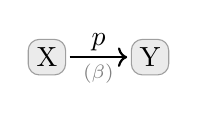
\begin{tikzpicture}[center base]
            \node[dpad0](X) {X};
            \node[dpad0,right=0.8 of X](Y) {Y};
            \draw[arr1](X) to
                node[above,inner sep=2pt]{$p$}
                node[below,inner sep=2pt]{${\scriptstyle\color{gray}(\beta)}$} (Y);
        \end{tikzpicture}
\]

It's extension is the update rule that incorporates data of the new PDG to the old one, where all confidences in the new PDG are scaled by $k$.
\[
    % F^{\beta}_{\dg M'}(\dg M) = \dg M ~+~ \beta\,\dg M'
    \bar F^{k}_{\dg M'}(\dg M) = \dg M ~+~ k\,\dg M'
\]

The natural update rule is
\[
    \bar G'_{\dg M'}(\dg M) = - \hat\nabla \aar{\dg M + \dg M'}
\]

\subsubsection{}
\begin{align*}
    \Theta :=
        \Big\{
        \text{PDGs over variables } \mat X
        \Big\}; \qquad
    \Phi := \Big\{
        \text{Probabilities}~ \mu \in \Delta \V(\mat X)
        \Big\}
\end{align*}


\subsubsection*{The Qualitative Half}


There are a number of different ways to think about alpha.
\begin{enumerate}[nosep]
    \item $\alpha_L$ is your confidence in the functional dependence of $Y$ on $X$, given
    \item $\alpha_L$ is the ``alignment'' of the edge $L$
\end{enumerate}

We need a different distance function for the other half. Now we use
$d(\mu, DET)$.

% \begin{align*}
%
% \end{align*}

We need a different distance function for the qualitative loss function of a PDG.
Why measure distance differently in this case?


\section{Relationships to Other Notions of Confidence}

\subsection{}

Define an update rule on $\Phi = \mathcal A$ via its vector field,
\[
    F'_A(\mu) := [ \mathbbm 1_{A} ]
     \qquad = x \mapsto \mathbbm1\{x \in A\} - \mu(A)
\]
which results in
\[
    F_A^\beta(\mu)(x) \propto
    \begin{cases}
        \mu(x) e^{-\beta} & x \in A \\
        \mu(x) & x \notin A
    \end{cases}
\]
\[\text{? or}\quad
    F_A^\beta(\mu) (B) =
    % \frac{1}{\Ex_\mu[ e^{} ]}
    \frac{1}{1 + (e^{-\beta}-1) \mu(A) } \mu(B) e^{-\beta \mu(A \cap B)}
\]

\subsection{Probability Measures}

% Fix a probability $\Pr(X)$, and
We began by remarking that often confidence is taken to mean probability.
With this framework in mind, here is one explanation why.

Suppose $F$ is an update rule for assertions $\Phi_F = \mathcal A$.
Now consider a modified update rule $\tilde F$ over assertions $\Phi_{\tilde F} = \Delta\X$, given in vector field representation as
% Fix a probability distribution $p(X)$.
% consider the update rule $G = \mathdcal F_p[F]$ whose vector field is given by
\[
    \tilde F'_p(\mu) := \sum_{x} p(x) F'_{\{x\}}(\mu)
    = \Ex_{x \sim p} [ F'_{\{x\}} (\mu) ].
\]

\subsection{Belief Functions}
More genrally, for the space of assertions $\Phi$ consisting of mass functions $m \in \Delta(2^X)$ that assign each subset of X, encoding a belief function. Then

\[
    \tilde F'_p(\mu) := \sum_{A \in \mathcal A} m(A) F'_{A}(\mu).
\]

% Intuitively, $\mathdcal F_p$ is the rule
% A fixed point of $\mathdcal F_p$ corresponds to an update rule such
% One natural question: what update rules



\subsection{Epistemic Entrenchment}
\subsection{Weighted Probability Measures}

\section{}
% Objective:
Consider a density $\rho : \X \to \mathbb R^+$, and consider the differential equations
\[
    % \frac{1}{u(x,t)}
    \frac{\mathrm d}{\mathrm d t} u(x,t)
    = - \Big\langle\mathrm d\beta(t), \ell(x) \Big\rangle
        \,
        {u(x,t)}
    \qquad\qquad%% OR %%%%%%%%%%%%%%%%%%%%%%%%%%%%%%%%%%%
    \dot {\mat u} = - \beta \mathrm{Diag}(\ell) \mat u
        % = - \Big\langle\mathrm d\beta(t), \ell(x) \Big\rangle
\]
Which means
\[
    % \Big|
        \log u (x,t)
    % \Big|
    = \int_{0}^{t}  \ell(x) \mathrm d \beta \mathrm d \tau
\]
% And suppose $C(t)$ is such that $u(x,t)$ is conserved, i.e.,





% \end{minipage}\label{ax:linear}\label{ax:linear}\label{ax:linear}\label{ax:linear}\label{ax:linear}\label{ax:linear}\label{ax:linear}





% What matters in the end are probabilities, as far as probabilistic models are concerned.
% But that doesn't mean that




% Probabilistic models may , but what matters in the end are probabilities.
In the opacity analogy, an update rule corresponds to a ``blending strategy'' --- a way of overlaying an image over another one, with a specified translucency.


\newpage
\printbibliography


\appendix
\section{General Thoughts}

\begin{itemize}
\item
(Variable) confidence is an important aspect of knowledge representation, because we need be able to entertain possibilities and reason about models we aren't sure about.

\item
Confidence is often thought of as the opposite of uncertainty.

\begin{itemize}
    \item
    Confidence is intimately related to probability, and our development will largely be couched in probabilistic terms. But they are not the same concept.
    While having high confidence in $\varphi$ is not so different from thinking $\varphi$ likely, having \emph{low confidence} in $\varphi$ is not the same as having thinking $\varphi$ is unlikely.
    To illustrate, consider a statement made by friend (a high-confidence source) and an adversary (a low-confidence source).

    \item
\end{itemize}

Rather, for us, it is \emph{conjugate} to uncertainty, in the way that force and distance are conjugate, and in the way that entropy and temperature are themodynamically conjugate variables.

Operationally, this means that it energetically unstable to have both high confidence and
% One has confidence in information.

\begin{wip}
! Why is $\mathit{Entropy} \cdot \mathit{Temperuature} = \mathit{Energy}$ but
 Why is $\mathit{Information} \cdot \mathit{Confidence} = \mathit{Energy}$ when confidence is like inverse temperature?
\end{wip}

\item
Confidence is, by nature, impossible to get an absolute scale for. This shows up again and again.
\begin{itemize}[nosep]
    \item PDG $\beta$ (and $\alpha$, relative to $\alpha_0$).
\end{itemize}

\item Confidence as inverse temperature.

\begin{itemize}
    \item
    ``cool-headed'' means calculated (a vote of confidence) while ``hot-headed'' means rash (such an assessment indicates a lack of confidence). Confidence is like inverse temperature.

    \item Boltzman rationality.
\end{itemize}


\item Confidence units: energy per inconsistency (at least when expressed as a gradient).

\item Pseudoinverse for constrained optimization
    \url{https://arxiv.org/pdf/1107.1944.pdf}

\item Geometrically, $\beta$ is the total distance to travel,

\item No Canonical Choice of Scale

\begin{itemize}
    \item Can choose choice of units to measure other things also (e.g., length in meters or feet).
\end{itemize}

\item Question:


\end{itemize}

% The notion of confidence also has
% Confidence is the opposite of uncertainty: you cannot be uncertain about $X$ .


% Confidence is dual to information.



Can you can be confident that $X$ is uncertain?
There is a huge difference between being certain that a coin has is fair, and knowing nothing about it.


% Here we draw a distinction between confidence and certainty:
% while you are certain that [proposition],




% Nevertheless, we submit that in many cases---and especially in more subjective or computationally restricted settings---probability alone is not enough, and the higher-order probabilistic picture is far too extreme.

Confidence as learning rate. Bigger confidence ~= bigger step size.
Learning algorithms have learning rate schedules (rates decrease or cycle).

\subsection*{Our Approach}
% Here is the idea: if you are confident in $X$, then you are
The idea is to view confidence as a property of an update, not as a property of a point of view.
In this telling

This allows us to distinguish between ...
%

% \begin{example}
% Let $X$ be a binary random variable, and suppose you have a prior probability $p$ that $X=1$.
% \begin{enumerate}
%     \item Suppose $p=1$.
%     This is a poor choice of prior.
%     If you then recieve information that $X=0$, something has gone very wrong, and the Bayesian update is undefined.
%
%     If you rceive information that $X = 1$, your internal state should not change.
%     % If we characterize
%
%     \item One might argue that only positive probabilities are relevant.
%     Suppose $p = 1 - \epsilon$.
% \end{enumerate}
% \end{example}


\subsection*{Issues To Address}
\begin{enumerate}
    \item The difference between having confidence in \emph{a source} and confidence in a particular \emph{fact}.  Is one more general than the other?
\end{enumerate}

Some intuitive features we might want to capture:
\begin{enumerate}

    \item \textbf{Trust Dynamics.} If a trusted source tells you something you already believe, your confidence in them goes up (maybe). Certainly if a source tells you something you know to be wrong, your confidence in the source goes down.  Whether or not you adopt the

    Also, if you ultimately end up adopting the belief, and later end upwith a more coherent picture of the world, your trust in the source should go way up.
    This is because in the end we want to place the most trust in sources that tell you the truth, not what you expect (or want) to hear.

    A source that tells you only exactly what you already believe ``artificially'' increases your confidence but does not actually provide you any information, unless they came to hold the same views independently.

\end{enumerate}

\TODO
\clearpage

\section{Useful Facts}
\begin{enumerate}
    \item Every length-minimizing curve in a Riemannian Manifold is a geodesic, if given a constant-speed parameterization
\end{enumerate}


\end{document}
